%% LyX 2.1.4 created this file.  For more info, see http://www.lyx.org/.
%% Do not edit unless you really know what you are doing.
\documentclass[11pt,czech,american]{book}
\usepackage[T1]{fontenc}
\usepackage[utf8]{inputenc}
\usepackage[a4paper]{geometry}
\geometry{verbose,tmargin=4cm,bmargin=3cm,lmargin=3cm,rmargin=2cm,headheight=0.8cm,headsep=1cm,footskip=0.5cm}
\pagestyle{headings}
\setcounter{secnumdepth}{3}
\usepackage{url}
\usepackage{amsmath}
\usepackage{amsthm}
\usepackage{amssymb}
\usepackage{graphicx}
\usepackage{setspace}
\usepackage[final]{pdfpages}
\usepackage{natbib}
\usepackage{mathrsfs}
\usepackage{algorithm}
\usepackage{algorithmicx}
\usepackage[noend]{algpseudocode}
\usepackage{caption}

\usepackage{array}
\usepackage{ragged2e}

\usepackage{lipsum}
\usepackage{psvectorian}

\DeclareMathOperator*{\argmax}{arg\,max}

\makeatletter
%%%%%%%%%%%%%%%%%%%%%%%%%%%%%% Textclass specific LaTeX commands.
\newenvironment{lyxlist}[1]
{\begin{list}{}
{\settowidth{\labelwidth}{#1}
 \setlength{\leftmargin}{\labelwidth}
 \addtolength{\leftmargin}{\labelsep}
 \renewcommand{\makelabel}[1]{##1\hfil}}}
{\end{list}}

%%%%%%%%%%%%%%%%%%%%%%%%%%%%%% User specified LaTeX commands.
%% Font setup: please leave the LyX font settings all set to 'default'
%% if you want to use any of these packages:

%% Use Times New Roman font for text and Belleek font for math
%% Please make sure that the 'esint' package is turned off in the
%% 'Math options' page.
\usepackage[varg]{txfonts}

%% Use Utopia text with Fourier-GUTenberg math
%\usepackage{fourier}

%% Bitstream Charter text with Math Design math
%\usepackage[charter]{mathdesign}

%%---------------------------------------------------------------------

%% Make the multiline figure/table captions indent so that the second
%% line "hangs" right below the first one.
%\usepackage[format=hang]{caption}

%% Indent even the first paragraph in each section
\usepackage{indentfirst}

%%---------------------------------------------------------------------

%% Disable page numbers in the TOC. LOF, LOT (TOC automatically
%% adds \thispagestyle{chapter} if not overriden
%\addtocontents{toc}{\protect\thispagestyle{empty}}
%\addtocontents{lof}{\protect\thispagestyle{empty}}
%\addtocontents{lot}{\protect\thispagestyle{empty}}

%% Shifts the top line of the TOC (not the title) 1cm upwards 
%% so that the whole TOC fits on 1 page. Additional page size
%% adjustment is performed at the point where the TOC
%% is inserted.
%\addtocontents{toc}{\protect\vspace{-1cm}}

%%---------------------------------------------------------------------

% completely avoid orphans (first lines of a new paragraph on the bottom of a page)
\clubpenalty=9500

% completely avoid widows (last lines of paragraph on a new page)
\widowpenalty=9500

% disable hyphenation of acronyms
\hyphenation{CDFA HARDI HiPPIES IKEM InterTrack MEGIDDO MIMD MPFA DICOM ASCLEPIOS MedInria}

%%---------------------------------------------------------------------

%% Print out all vectors in bold type instead of printing an arrow above them
\renewcommand{\vec}[1]{\boldsymbol{#1}}

% Replace standard \cite by the parenthetical variant \citep
%\renewcommand{\cite}{\citep}

\makeatother

\usepackage{babel}

\newcommand{\ornamentleft}{%
	\psvectorian[width=2em]{2}%
}
\newcommand{\ornamentright}{%
	\psvectorian[width=2em,mirror]{2}%
}

\newcommand{\ornamentheader}[1]{%
	\begin{center}
		\ornamentleft
		\quad{\large\emph{#1}}\quad % style as desired
		\ornamentright
	\end{center}%
}

\newlength{\rlength}\setlength{\rlength}{16cm}
\newcommand{\ruletext}[2][\rlength]{%
	\noindent%
	\parbox{#1}{%
		\noindent\dotfill\raisebox{-.3\ht\strutbox}{#2}\dotfill\par}%
}





\begin{document}
\def\documentdate{July 7, 2017}

\newtheorem{definition}{Definition}[chapter]
\newtheorem{note}{Note}[chapter]
\newtheorem{example}{Example} 
\newtheorem{assumption}{Assumption} 

\newtheorem{theorem}{Theorem}
\newtheorem*{remark}{Remark}

\captionsetup[figure]{labelfont={bf},labelformat={default},labelsep=period,name={Fig.}}

\def\documentdate{\today}

\pagestyle{empty}
{\centering

\noindent %
\begin{minipage}[c]{3cm}%
\noindent \begin{center}

\includegraphics[width=3cm,height=3cm,keepaspectratio]{Images/TITLE/cvut}
\par\end{center}%
\end{minipage}%
\begin{minipage}[c]{0.6\linewidth}%
\begin{center}
\textsc{\large{}Czech Technical University in Prague}{\large{}}\\
{\large{}Faculty of Nuclear Sciences and Physical Engineering}
\par\end{center}%
\end{minipage}%
\begin{minipage}[c]{3cm}%
\noindent \begin{center}

\includegraphics[width=3cm,height=3cm,keepaspectratio]{Images/TITLE/fjfi}
\par\end{center}%
\end{minipage}

\vspace{3cm}


\textbf{\huge{}Real Options Valuation: A Dynamic Programming Approach}{\huge \par}

\vspace{1cm}


\selectlanguage{czech}%
\textbf{\huge{}Oceňování projektů metodou reálných opcí z pohledu dynamického progamování}{\huge \par}

\selectlanguage{american}%
\vspace{2cm}


{\large{}Master's Thesis}{\large \par}

}

\vfill{}

\begin{lyxlist}{MMMMMMMMM}
\begin{singlespace}
\item [{Author:}] \textbf{Filip Rolenec}
\item [{Supervisor:}] \textbf{Ing. Rudolf Kulhavý, DrSc.}
\end{singlespace}

\item [{Language~advisor:}] \textbf{Ing. Rudolf Kulhavý, DrSc.} 
\begin{singlespace}
\item [{Academic~year:}] 2020/2021\end{singlespace}

\end{lyxlist}
\newpage{}

~\newpage{}

~

\vfill{}


\begin{center}
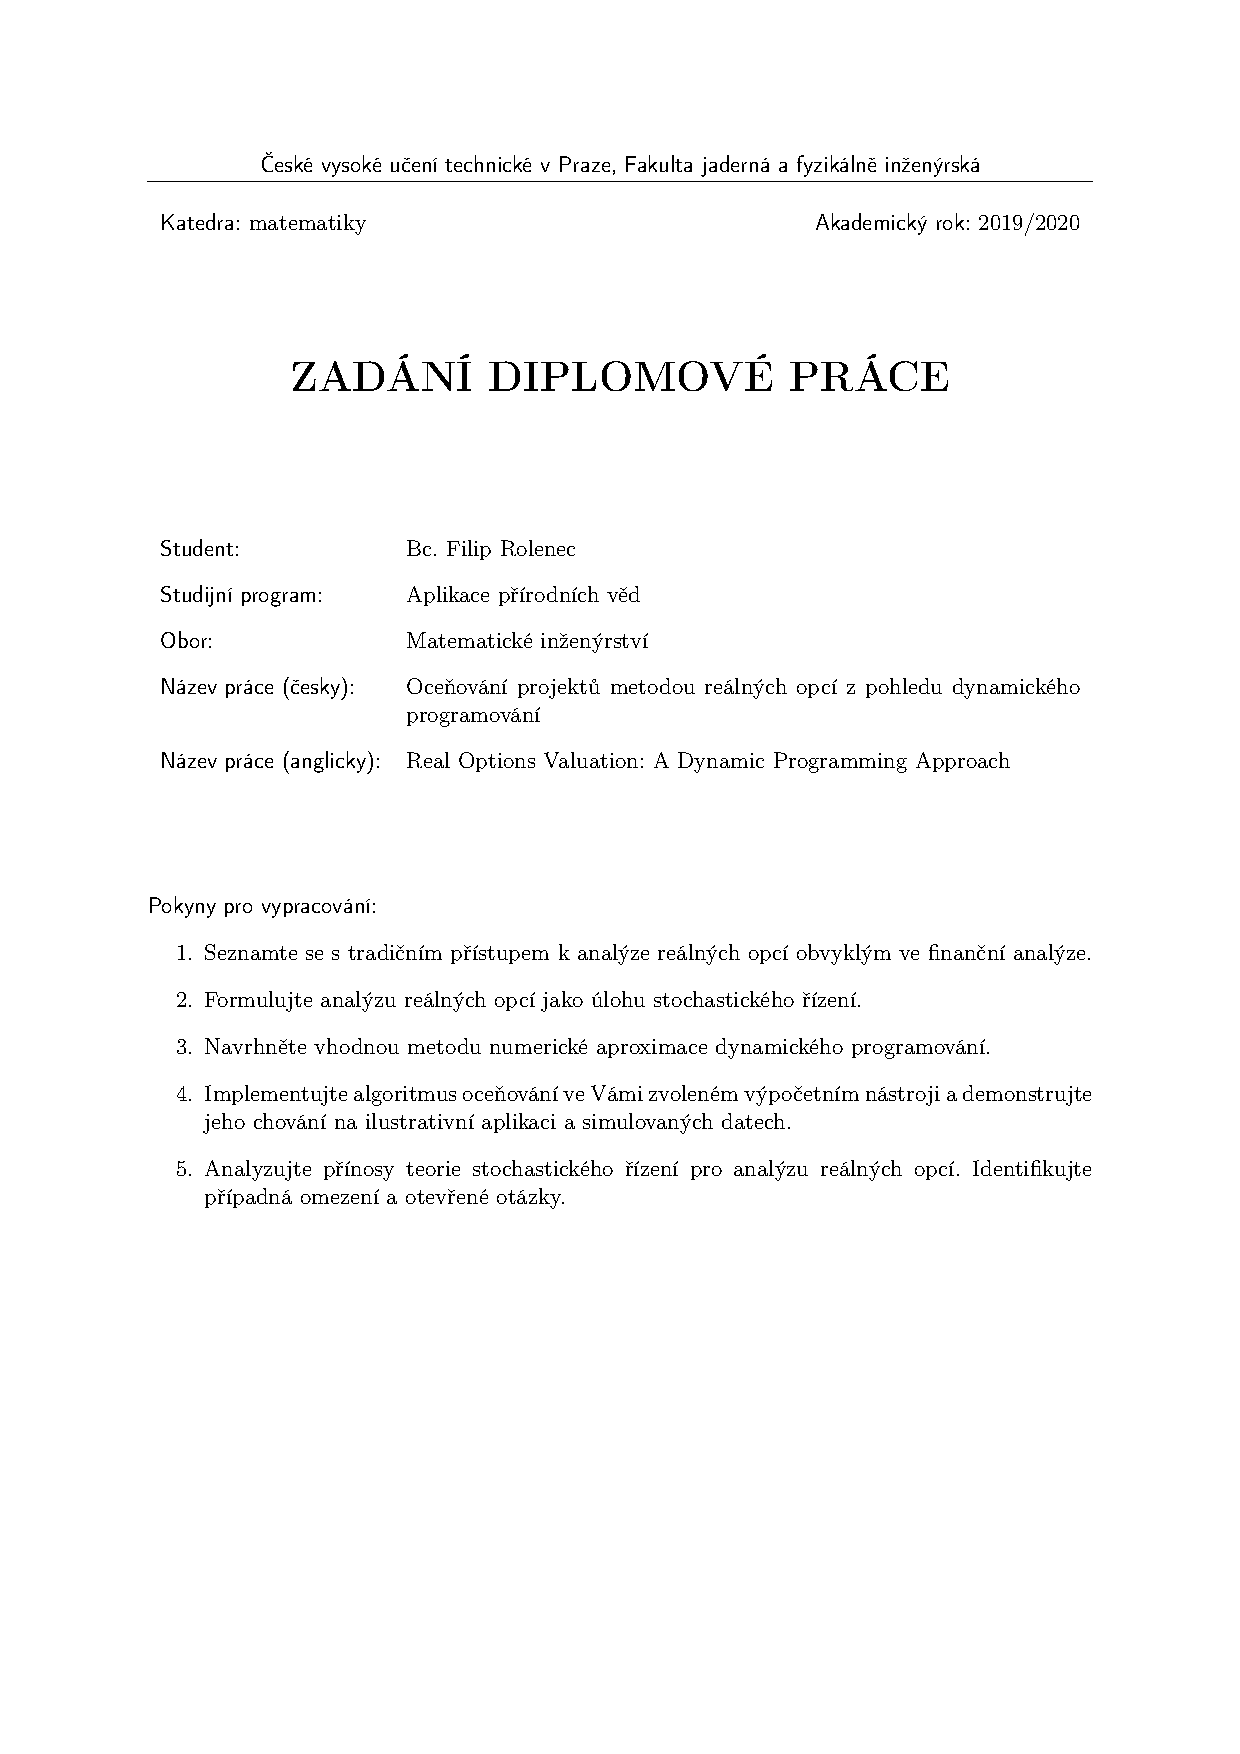
\includepdf[pages={1}]{Images/zadaniMT.pdf}


\par\end{center}

\vfill{}


~\newpage{}

~

\vfill{}


\begin{center}
\includepdf[pages={2}]{Images/zadaniMT.pdf}
\par\end{center}

\vfill{}


~\newpage{}

\noindent \emph{\Large{}Acknowledgment:}{\Large \par}

\noindent I would like to thank my supervisor Ing. Rudolf Kulhavý, DrSc. for his professional guidance and all the advice given while creating this thesis. 

\vfill

\noindent \emph{\Large{}Author's declaration:}{\Large \par}

\noindent I declare that this Master's thesis is entirely
my own work and I have listed all the used sources in the bibliography.

\bigskip{}


\noindent Prague, \documentdate\hfill{}Bc. Filip Rolenec

\vspace{2cm}


\newpage{}

~\newpage{}

\selectlanguage{czech}%
\begin{onehalfspace}
\noindent \emph{Název práce:}

\noindent \textbf{Oceňování projektů metodou reálných opcí z pohledu dynamického progamování}
\end{onehalfspace}

\bigskip{}


\noindent \emph{Autor:} Bc. Filip Rolenec

\bigskip{}


\noindent \emph{Obor:} Matematické inženýrství 


\bigskip{}


\noindent \emph{Druh práce:} Diplomová práce

\bigskip{}


\noindent \emph{Vedoucí práce:} Ing. Rudolf Kulhavý, DrSc.


\bigskip{}


\noindent \emph{Abstrakt:} \textbf{BUDE DOPLNĚNO }


\bigskip{}


\noindent \emph{Klíčová slova:}   Analýza reálných opcí, Blackův-Scholesův model, Čistá současná hodnota, Dynamické programování, Energetika, Oceňování projektů, Stochastická rozhodovací teorie



\selectlanguage{american}%
\vfill{}
~

\begin{onehalfspace}
\noindent \emph{Title:}

\noindent \textbf{Real Options Valuation: A Dynamic Programming Approach}
\end{onehalfspace}

\bigskip{}


\noindent \emph{Author:} Bc. Filip Rolenec

\bigskip{}


\noindent \emph{Abstract:} \textbf{WILL BE ADDED}
	
	
\bigskip{}


\noindent \emph{Keywords:} Black-Scholes model, Dynamic programming, Net present value, Power industry, Project valuation,  Real option analysis, Stochastic decision control

\newpage{}

~\newpage{}

\pagestyle{plain}

\tableofcontents{}

\newpage{}


\chapter{Historical background and research motivation}
The foundations of financial derivatives date back to the origins of commerce in Mesopotamia in the fourth millennium BC \cite{Web:09}. The derivative market consisted mainly of forward contracts \footnote{A forward contract is a contract to purchase an asset at a fixed price on a particular date in the future. \cite{BerDeM:09} } and it was introduced to the European continent through Spain in Roman times. After the expulsion of derivative trading in Spain the center of this type of commerce for Europe were the Low Lands, where at the end of the 17th century, the first ideas about options \footnote{A financial option is the \textbf{ability} to buy (call option) or sell (put option) a defined volume of an asset for a specified amount of money in a given future time instant. \cite{BerDeM:09}}  and option trading are published by La Vega \cite{Veg:88}. 

The first attempts of a mathematical option pricing come from Bachelier (1900) \cite{Bac:00} and Bronzin  (1908) \cite{Bro:08}. Based on their work, the boom of option pricing methods in the 1970's culminated in Nobel-price-winning Black-Scholes model \cite{BlaSch:73}, which is today's standard in the option pricing theory\cite{YalHak:12}. 

The publicity and wide adoption of the BSM model most likely inspired an expert on capital budgeting, Stewart Myers, to introduce the term "Real Options" \cite{Mye:77}, one of two main pillars of this thesis. Myers builds on the idea that part of the project's value is hidden in the form of real options - the ability to change the course of the project in the future. Myers' approach to the real options is mostly philosophical in the sense that he stresses the importance of thinking about the additional value options bring. At the same time he does not present any computational tool for the said value. 

The idea of Real Option Analysis (ROA) as a valuation tool for projects was further developed by several influential authors in the following decades, for example Guthrie \cite{Gut:09}, Vollert \cite{Vol:03} Pindyck \cite{DixPin:12} and Kulatilaka \cite{AmrKul:98}. 

The valuation of project's free cash flows with the theory of ROA is in the economic world understood as very advanced, and its adoption in practice is slow \cite{Amp:17}. It is argued that this slow adoption is caused mainly by misunderstanding the more difficult mathematical concept of ROA \cite{SicGam:10} and the low adoption rate of a competition: "Why should our company use a new tool that no one else is using?" \cite{CopAnt:01}. 

Through the study of the ROA state of the art, we have identified that there is a discrepancy in understanding what ROA actually is. As will be illustrated in-depth in section ... we identify three classes of ROA authors based on the level of analogy to the BSM model. 

In this thesis, we focus on the second class of ROA authors represented by brilliant publications of Graeme Guthrie \cite{Gut:09} and Alexander Vollert \cite{Vol:03}.\footnote{Second class utilizes only the no-arbitrage principle to determine the probabilities of the models.}  

Through my studies at the FNSPE CTU, I have specialized in the theory of dynamic decision making under uncertainty \cite{Rol:18}, \cite{Rol:19}. When studying ROA it came only natural to understand the project valuation as an optimal decision making problem. 

The goal of this thesis is to take the project valuation problem structure as is understood in ROA and look at it from the perspective of stochastic decision theory (SDT). One of the challenges of this task is to implement domain-specific economical truths about investors' behavior and the way they perceive value.  Two main addressed concepts are the time value of money and the risk aversion of investors. 

The goal of this thesis is to provide an SDT-based valuation algorithm for projects, whose value is understood as a maximal possible current cash equivalent of the uncertain future cash flows. This valuation algorithm will cover the classes of problems now solved by ROA and allow for new ones. 

The new SDT based valuation algorithm will enable: 
\begin{itemize}
	\item seamless integration of multiple uncertainty sources;
	\item integration of theoretically any probability distribution as a model of uncertain variables;
	\item usage of a high number of possible actions, regardless of their nature; 
	\item utilization of approximate dynamic programming tools for high-dimensional problems;
	\item preservation of the economic truths as time value of money and the risk aversion of investors. 
\end{itemize}

To illustrate the usage of the new SDT-based algorithm a valuation of a project from a selected class is performed. This class is denoted as \textit{facilities with simple input-output process models}. It covers all projects whose cycle time is equal to zero, and the input-output transformation rate is constant. This class is a generalization motivated by an example of gas power plant valuation presented by Guthrie in \cite{Gut:09}. 


The thesis is structured into 5 chapters. Chapter 1 reminds the reader of the most important mathematical and economic concepts used in this thesis. Beginning with the declaration of mathematical notation, the chapter continues with key concepts of economic theory and a deeper description of the BSM model. The first chapter continues with a summary of the last decades in ROA research, focusing on a specific level of analogy represented by Vollert \cite{Vol:03} and Guthrie \cite{Gut:09}. The remainder of the first chapter is reserved for key parts of stochastic decision theory. 

Chapter 2 represents the core of this thesis. First, we define what will be understood as a problem of ROA project valuation. We state the key features that define a project,and we limit these features accordingly (?). Then we focus on the interpretation of the problem by a general SDT framework. We illustrate the identification of ROA project features in SDT. The remainder of the second chapter is reserved for resolving the economic nuances that need to be accounted for in the SDT framework in order to make the valuation procedure consistent with the economic reality of investors' behavior. 

Chapter 3 illustrates the new valuation algorithm from chapter 2 on an example of valuation of a facility with a simple input-output process model. A valuation of a gas power plant is chosen as the representative of this class. The first half of the chapter focuses on the value sensitivity with regard to the volume of available managerial actions in the project. The second half presents a value comparison  of project alternations in different granularity of the model structure and it is aimed to demonstrate the existence of trade-of between computational complexity and precision of computed results. 

Chapter 4 discusses the new findings, both theoretical and observed from the performed experiments. 

Chapter 5 summarizes the thesis - reminds the motivation, underlines the main message, and lists all contributions of this thesis. Furthermore, it outlines many possible future research paths in this field as it is, to our best knowledge, the first available publication on this topic. 


%\addcontentsline{toc}{chapter}{Introduction}

%\addcontentsline{toc}{chapter}{Preliminaries}

\pagestyle{headings}




\chapter{Preliminaries}
To properly understand a mathematical text it is important to first define the used notions and symbolism. Since this thesis is based on many different authors, from both financial and mathematical world, a short unifying overview of the used theory is important. 

The notation used in this thesis comes predominantly from the most influential authors in the respective fields of study: 
\begin{itemize}
	\item general economy \cite{BerDeM:09};
	\item real options \cite{Gut:09};
	\item stochastic decision theory \cite{BacChi:19}.
\end{itemize}

 The pure mathematical symbolism comes from the author's studying experience at FNSPE CTU and its proven applicability in his previous publications \cite{Rol:18} and \cite{Rol:19}. 


\section{General mathematics}
In the whole thesis, bold capital letters, such as $\mathbf{X}$, represent a set of all elements $x \in \mathbf{X}$ as in \cite{Rol:18}. The cardinality of a set $\mathbf{X}$ is denoted with two vertical lines as $|\mathbf{X}|$. Random variables, understood in a sense of the standard Kolmogorov's probability theory \cite{Kol:60}\footnote{Does this citation make sense?}, are represented with a tilde above the variable, i.e. $\tilde{x}$. Realizations of random variables are denoted by the same letters as the random variable without the tilde, i.e. $x$. 

\begin{definition}(Probability)
	Let $\tilde{x}$ be a random discrete variable. Then $P(x)$ denotes a probability that the realization of $\tilde{x}=x$. Similarly if $\tilde{x}$ is a continuous random variable, then $p(x)$ denotes a probability density of the realization $\tilde{x}=x$. 
\end{definition}
\begin{remark}
	To rigorously unify the notation and simplify the formulas a Radon-Nikodým (RN) density \cite{Rao:87a} is introduced  with the notation $p(x)$ and the name ``probability density``. The dominating measure of this RN density is either the counting measure (in discrete case) or the Lebesgue measure (in continuous case). The notation $P(X)$ is reserved only for the cases when the discreteness of the argument needs to be emphasized. 
\end{remark}

The last general definition is the definition of well known concept of conditional probability \cite{Jay:03}. 
\begin{definition}(Conditional probability)
	Let, depending on the context, symbol $p(x|y)$ represent the conditional probability density of a random variable variables. Then the $p(x|y)$ is defined as:
	\begin{equation}\label{eq:condP}
	p(x|y)=\frac{p(x,y)}{p(y)},
	\end{equation} where $p(x,y)$ is a joint probability density of $\tilde{x}$ and $\tilde{y}$. 
\end{definition}

\begin{remark}
	The definition of conditional probability expressed by the equation (\ref{eq:condP}) corresponds with the classic definitions of the conditional probability and conditional probability density in both the discrete and continuous case. 
\end{remark}

\begin{definition}(Expected value)
	Expected value of a random variable $\tilde{x}$ is defined as: 
	\begin{equation}
		\int_{\mathbf{X}} p(x) x d\mu,
	\end{equation}
	where $\mu$ is the dominating measure of the RN density and $\mathbf{X}$ is the set of all possible realizations of $\tilde{x}$.
\end{definition}
<Probably some other definitions that will be needed in the following chapters >

\subsection{Probability distributions}
Thorough this thesis more advanced distribution will be referenced, either as an expected model of some random variable, or in a broader discussion. The following non-trivial probability distributions are important for this thesis \cite{Bli:19}. 

\paragraph{Bernoulli distribution}
The most simple non-trivial distribution is the Bernoulli distribution $Be(p)$, which models the probability of success (1) or failure (0) with $p \in [0,1]$: 

\begin{equation}
p(\tilde{x} = x) =
\left\{
\begin{array}{ll}
p  & x=1\\
1-p & x=0.
\end{array}
\right.
\end{equation}

This distribution is seemingly the most used in the modeling of uncertainty in the ROA theory. It usually models the up (1) and down (0) movement of asset or commodity prices. 


\paragraph{Binomial distribution}
Binomial distribution $Bi(n,p)$ represents the number of successes of $n$ independent random variables distributed by $Be(p)$ as:

\begin{equation}
	p(\tilde{x}=k)=\binom{n}{k} \cdot p^k(1-p)^{n-k}.
\end{equation}

As a logical result, the binomial distribution in ROA models the asset or commodity prices after $n$ time intervals. 


\paragraph{Poisson distribution}
Poisson distribution $Po(\lambda)$ is a popular discrete distribution used in modeling of number of successes in a given time-interval, so called ``arrivals`` \cite{Bli:19}. It is used for modeling of number of incoming emails or number of earthquakes in given area in one year. 

Its probability density function PDF given parameter $\lambda$ is: 
\begin{equation}
	p(\tilde{x}=x)= \frac{\lambda^xe^{-\lambda}}{x!} , 
\end{equation}
where $x\in \mathbb{N_0}$.

Also, it is worth noting that Poisson distribution $Po(\lambda)$ with $\lambda = np$ is the limit distribution of a $Bi(n, p)$ for $n \to \infty$. 


\paragraph{Log-normal distribution}
Another very popular distribution in the ROA theory is the log-normal distribution $LogN(
\mu, \sigma)$. It represent a random variable, logarithm of which is distributed normally. 

The probability density function of such variable is:
\begin{equation}
	p(\tilde{x}=x)=\frac{1}{x\sigma\sqrt{2\pi}} exp\left(\-\frac{(ln(x)-\mu)^2}{2\sigma^2}\right).
\end{equation}

This distribution is used again mostly for modeling of asset or commodity prices.And it has two pleasant properties. First, that its realizations are positive and  second, that variance reflects not only the parameter $\sigma$, but also $\mu$, where $\mu$ usually represents the previous price. 



\section{General economics}

This thesis is built on two main theoretical pillars, the theory of corporate finance \cite{BerDeM:09} and stochastic decision theory (SDT) \cite{BacChi:19}. A basic review of corporate finance terminology is presented in this section with a focus on project valuation techniques. 


\begin{definition}(\textbf{Process})
	A process is understood as the production of goods, purchase and trade of goods or services, driven by the supply of inputs and demand for outputs. \footnote{How to cite Mr. Kulhavy? }
\end{definition}

\begin{definition}(\textbf{Project})
	A project is defined as an sequence of actions that serve as an implementation or a innovation of a process, purposefully allocating existing sources to increase the economical value of given project.  
\end{definition}

\begin{definition}(\textbf{Free cash flow})
	The incremental effect of a project on the firm’s available cash is the project’s free cash flow \cite{BerDeM:09}.
\end{definition}


\begin{definition}(\textbf{Economical value})
	An economical value of a project is understood to be in the future free cash flows. In this thesis the economical value of a project is the amount of cash to which is the investor logically indifferent to having in comparison to the future cash flow vector. 
\end{definition}

\begin{remark}
	The indifference and time value of money will be further discussed in section ... The theory of net present value (NPV) \cite{BerDeM:09} can be used as a simplification. 
\end{remark}

\begin{definition}(\textbf{Optimal Project})
		The goal of each project is to increase the economical value of a process. A project, if such exists, is called optimal project if the additional economical value is maximal given the set of possible projects. 
\end{definition}


\subsection{Net present value}
Net present value is an industry standard valuation technique in capital investment. It is simple and it reflects the time value of money by exponential discounting of the future cash flow by a constant dicount rate $r$ (usually a risk-free interest rate): 

\begin{equation}
NPV(C) = \sum_{t \in \mathbf{T}} \frac{c_t}{r^t}, 
\end{equation}

where $C$ is a cash flow vector with its elements $c_t, t \in \{0,1,...,|C|\}$. 

This basic form of the NPV technique is a first approximation of the real current value of cash flow vector $C$, which means that its reflection of reality is rather limited. 

In this thesis we want to challenge the problem of constant discounting of positive and negative cash flow, which implies that the investor is able to invest in risk-free assets at the same rate at which he is able to borrow money. This is however, far from the reality. 

We challenge this problem in the next section by presenting the present cash equivalent metric. 


\subsection{Present cash equivalent}
The ability to borrow money for a given interest rate $r_b$ is individual for each investor and naturally different from the risk-free interest rate $r_r$. This asymetry is not reflected in the standard NPV metric and thus we come up with our own metric, which we call present cash equivalent, PCE. 

The notion of PCE is based on the logical indifference of an investor to a vector of future cash flow and some current amount of money. 

For the purpose of PCE lets prepare also the notion of so called responsible manager (RM).  The task of RM is to reinvest the positive balance (with the rate $r_r$) and borrow more funds in case of negative balance for the rate of $r_b$. 

We represent this behavior by the RM function, where the constant rates are not explicitely denoted, but rather implicitely assumed: 

\begin{equation}
RM(b) = 
\left\{
\begin{array}{ll}
b\cdot(1+r_r)  &  \mbox{if } b\geq 0 \\
b\cdot(1+r_b)  & \mbox{otherwise}
\end{array}
\right.
\end{equation}

Then, based on the assumption of completely dynamic loans\footnote{Meaning that bank will lend us money at any time and also will accept repayments at any time, all with the same interest rate.} we model the behavior of $RM = RM_{r_r,r_b}$ on a given cash flow vector $C = \{c_0,...c_t\} \ t \in \mathbb{N}$ as: 

\begin{equation}
	RM(C) = RM(...RM(RM(c_0)+c1)...+c_t). 
\end{equation}

The amount of $RM(C)$ represents the amount of money at time $t$ obtained from the cash flow vector $C$ and a logical money management. Then, the PCE(C) can be finally derived as: 


\begin{equation}
	PCE(C) = 
	\left\{
	\arraycolsep=5pt\def\arraystretch{1.5}
	\begin{array}{ll}
	\frac{RM(C)}{(1+r_r)^{t}}  &  \mbox{if } RM(C)\geq 0 \\
		\frac{RM(C)}{(1+r_b)^{t}}  &  \mbox{otherwise} 
	\end{array}
	\right.
\end{equation}


which represents the logic, that having PCE(C) at time $t =0$ would result in the same outcome at time $t$. Thus, a manager should be logically indifferent to obtaining $PCE(C)$ now and $C$ by its parts in different times. 

\subsection{Risk averse investors}\label{sec:risk_aversion_preliminaries}
According to the observations made in \cite{BerDeM:09} there is a positive correlation between the volatility of an investment and its average profit. This correlation is being explained by the risk aversion of investors, where investors are happy to hold onto a low-volatile investment even though the average returns are lower in the long run. 

The phenomenon of risk aversion is well documented also in psychological publications, i.e. \cite{HolLau:05}, where we observe that people do not like uncertainty and they do value uncertain rewards lower than their expected value. 

\subsection{Option valuation - Black-Scholes-Merton model}
As outlined in the first chapter, the motivation for option valuation technique came  with the increased adoption of derivative trading after the WWII. The famous 1973 article from Black and Scholes \cite{BlaSch:73} presented today's standard in the option valuation - the BSM model. 

\begin{remark}
	The M in BSM model stands for Merton, as the publication of Black and Scholes ``relied on earlier work by Robert Merton.``  \footnote{I want to talk about it because I want to explain why BSM and not BS model, where I do not want to use BS model for obvious reasons. }
\end{remark}

In what follows we will present the BSM model in a form of a theorem \cite{BodKan:04}. In addition we will present an opinion that should summarize the idea of BSM model in few sentences. 

\begin{theorem}(BSM model)
	The Black-Scholes-Merton option valuation model says that if the following list of assumption is satisfied:
	\begin{itemize}
		\item risk-free interest rate and volatility of the underlying asset are constant;
		\item the underlying asset pays no dividends and its price is continuous;
		\item the asset price evolves according to a log-normal process;
		\item the markets are efficient - the no-arbitrage principle holds;
		\item the option has European style;
		\item there are no commission or transaction costs;
		\item market is perfectly liquid;
	\end{itemize}

	then based only on the knowledge of time to maturity $T$, option's strike price $K$, the current price of underlying asset $S$ and its volatility $\sigma$ the value of a call option can be computed as: 
	\begin{equation}
	C = SN(d_1) - PV(K)N(d_2), 
	\label{BSMModelEq}
	\end{equation}
	where  $PV(K)$ is the present value of a strike price $K$ \footnote{Price of a bond paying K on the expiration day of the option} and $N(d)$ is a cumulative normal distribution, probability that a normally distributed variable is less than $d$. Value of $d_1$ and $d_2$ is then defined as: 
	\begin{equation}
	d_1 = \frac{ln(S/PV(K))}{\sigma \sqrt{T}}+\frac{\sigma \sqrt{T}}{2}  \quad
	d_2 = d_1 - \sigma \sqrt{T}
	\end{equation}
\end{theorem}

\begin{remark}
	The dependency of the price of an option is positive in case of volatility and time to maturity Increasing these parameters leads to a higher option price. On the contrary the rise in current stock price or strike price of the options lowers the value of an option. 
\end{remark}

Now, we would like to present our opinion about what the BSM model actually says. 

\begin{remark}
	The core of BSM model, assuming that "smooth" conditions hold, represents a way to derive a parameter in a log-normal model of the underlying asset. Based on the no-arbitrage principle and assumption of known volatility $\sigma$, only the parameter $\mu$ of log-normal process is missing. Building on this, the value of an option is the expected value of the maximum of difference between strike price and the realized price of the asset and zero \footnote{Since the option does not have to be realized, no further loss will occur.}, discounted by the risk-free interest rate. 
\end{remark}


\section{Real option analysis}\label{sec:ROA}
As outlined in the first chapter, the theory of real option analysis (ROA) was born after the boom in publications about valuation of financial options in the 1970's. The first ideas represented by Myers \cite{Mye:77} are of a philosophical nature - options (ability to make project changes) adds value to the project. 

Many publications were published on the ROA topic since. Through our studies of the state of the art, we have identified three classes of authors which differ by the level of analogy with the BSM model. 


\paragraph{No analogy}
The first class is the class of the ROA founder, Myers. This class understands the term real option analysis as a useful lens for looking at the project valuation. Authors like \cite{Kas:04} and \cite{Gue:17} accentuate the value of further managerial decisions, but the valuation strategy they use is NPV with scenarios (so called decision tree analysis DTA). 

\paragraph{Partial analogy}
The second class of authors takes advantage of the core property of the financial option valuation and that is the no-arbitrage principle. Based on this principle and further assumption of replication portfolio existence, this class of authors, e.g. \cite{Gut:09}, \cite{Tho:19} and \cite{Ryu:17}, derives so called risk-neutral probabilities, which are then used for modeling of some project's internal variable of the cash flow functions. 

Because we find this type of approach to real options as the most appropriate one and because we build on and respect the work of Guthrie \cite{Gut:09}, \textbf{this approach is the one considered as representative of the term ROA. }

Another author in this class whose work is notable is publication \cite{Vol:03} from Vollert, who goes deep into detail with modeling framework implementing complex conditional options. Vollert's publication is very advanced, using i.e. stochastic differential equations, which might be an obstacle for practitioners and real world applications.  

\paragraph{Full analogy}
The final class of the authors understands project valuation with real options as a complete analogy to the BSM model for valuation of financial options. This class of authors is predominantly represented by voluminous economical textbooks, e.g. \cite{BerDeM:09}, \cite{BreMye:12} or \cite{Cru:08}\footnote{Crundwell also discusses the partial analogy approach in detail.}. 

A complete analogy means to identify all parameters of financial option with a parameter of investment. For example in \cite{BerDeM:09} the following identification table is presented: 


\begin{table}[H]
	\begin{footnotesize}
		\centering
		\renewcommand{\arraystretch}{1,2}
		\label{Tab:BSModel}
		\begin{tabular}{|l |r|}
			\hline	
			Financial option& Real option \\ \hline
			Stock price& Current market value of asset \\ \hline
			Strike price& Upfront investment required	\\ \hline
			Expiration date& Final decision date \\ \hline
			Risk-free rate& Risk-free rate\\ \hline
			Volatility of stock & Volatility of asset value \\ \hline
			Dividend\footnotemark & FCF lost from delay \\ \hline
		\end{tabular}
		\caption{Identification of parameters for real options with respect to the financial option \cite{BerDeM:09}. }
	\end{footnotesize}
\end{table}
\footnotetext{For the BSM model with dividends}

Another example can be found in \cite{Que:10}, where a telecommunication company is being valued by the same one-to-one identification of BSM model parameters. 

By focusing on the complete analogy, the authors of this class strictly limit the application scope of the ROA valuation technique (as they understand it). One of the problematic assumptions (that is in the partial-analogy class solved by the CAMP model \footnote{Capital Asset Pricing model - for details please see \cite{Gut:09}}) is that there exists a market tradeable replicating portfolio of the asset we want to valuate. Another limitation is that this approach considers only one decision, which is usually to invest in the project now, or later \footnote{Timing option in Guthrie's terminology}. 

\vspace{1em}

In what follows, our understanding of ROA will be based on the one presented by Guthrie. This decision is based on the exceptionality of his publication \cite{Gut:09}. A rigorous definition of ROA as we will understand it will be presented in the beginning of the following chapter. 


\section{Statistical decision theory}
The second pillar upon which this thesis stands is the statistical decision theory (SDT). An area of applied mathematics that formalizes and studies optimal decision making of agents. As decision making under uncertainty in its broadest sense encapsulates the majority of human behavior, the class of problems it is able to solve (at least theoretically) is quite large. 

The SDT's main focus is to determine the optimal strategy (a sequence of decisions) to act upon, generally in dynamic and uncertain environment. In this thesis we will be modeling the decision making problems by the standard framework of Markov Decision Process (MDP).

\begin{definition}(Markov decision process)
	
	Markov decision process is defined by its five building blocks: 
	\begin{itemize}
		\item Set of time epochs - $\mathbf{T}$;
		\item Set of states in those epochs - $\mathbf{S_t}$, $t \in \mathbf{T}$;
		\item Set of actions in those states - $\mathbf{A_{s_t}}$, $s_t \in \mathbf{S_t}$, $t \in \mathbf{T}$;
		\item Reward function of transition from one state to another - $r(s_t|a_t,s_{t-1})$, where $s_t, \in \mathbf{S_t}$, $s_{t-1}, \in \mathbf{S_{t-1}}$,  and $a_t \in \mathbf{A_{s_t}}$;
		\item Transition probabilities governing the transitions from one state to another $p(s_t|a_t,s_{t-1})$, where $s_t, \in \mathbf{S_t}$, $s_{t-1}, \in \mathbf{S_{t-1}}$,  and $a_t \in \mathbf{A_{s_t}}$;
	\end{itemize}
\end{definition}

\begin{remark}
	The set of time epochs, states, actions is usually known, defined by the structure of the decision problem that is being solved. Reward and transition functions tend to be unknown in solving these problems and they need to be often somehow estimated. 
\end{remark}

\begin{remark}
	For further simplification of the text, we define $\mathbf{S} = \bigcup\limits_{t \in \mathbf{T}} \mathbf{S_t}$ and $\mathbf{A} = \bigcup\limits_{s \in \mathbf{S}} \mathbf{A_{s}}$.
\end{remark}


Usually, the biggest task in SDT is to correctly approach the uncertainty about transition probabilities between the different states of a decision making problem. There are two approaches to parameter estimation in statistics, classical approach and a Bayesian approach. Since the Bayesian approach seems to fit the format of decision making better - allowing for notion of prior probabilities, incorporating experts knowledge and possibility for smooth updating on newly observed data - it is used in this thesis. 

As outlined above, the goal of SDT is to find the optimal strategy - sequence of actions. The optimality of such strategy is defined as it having the maximal expected cumulative reward among all eligible strategies $\mathbf{\Pi}$: 

\begin{equation}
	\pi^*=\argmax_{\pi \in \mathbf{\Pi}} E\left[\sum_{t\in \mathbf{T}} r(s_t|a_t,s_{t-1})|\pi\right].
\end{equation}

\begin{remark}
	This definition of optimal strategy is used mainly in finite decision problems or problems with exponential discounting of future rewards. Alternative definitions of optimality, for example maximal average reward per period, exist.
\end{remark}

 Due to the nature of project valuation, where projects are considered to be finite or their cash flow exponentially discounted, this thesis will focus on the total cumulative reward.  

\subsection{Dynamic programming}
Finding the optimal policy by computing the expected reward for all policies $\pi \in \mathbf{\Pi}$ is due to the cardinality of $\mathbf{\Pi}$: 
\begin{equation}
|\mathbf{\Pi}|= \prod_{t\in\mathbf{T}} \prod_{s_t \in \mathbf{S_t}} |\mathbf{A_{s_t}}| 
\end{equation}  
very demanding task even for low-dimensional problems. 


To cope with such computational complexity a clever idea of backward induction, called dynamic programming, is used. The core of dynamic programming is to define so called value function $V(s)$ on each of the possible states $s \in \mathbf{S}$. Each of the values is computed via the Bellman equation: 
\begin{equation}\label{eq:Bellman}
V(s_{t-1}) = \max_{a_{t-1} \in \mathbf{A_{s_{t-1}}}}\sum_{s_t \in \mathbf{S_t}} p(s_t|a_t, s_{t-1}) [r(s_t|a_t, s_{t-1})+V(s_t)].
\end{equation}

Value function represents the expected cumulative reward from given state onward. The idea of computing this value through the backward induction is based on the truth that a sequence of actions is optimal if and only if the last action is optimal.  Optimal strategy comes together with the value function seemingly as a byproduct, where in each state, the optimal action is the argmax of the expression in equation \ref{eq:Bellman}. 

This clever approach significantly reduces the computational complexity to
\begin{equation}
	\sum_{t \in \mathbf{T}} \sum_{s_t \in \mathbf{S_t}} |\mathbf{A_{s_t}}|
\end{equation}
expected values. 

\begin{remark}
	For constant number of states and actions in each time epoch, this reduction is from $|\mathbf{T}|^{|\mathbf{S_t}|^{|\mathbf{A_{s_t}}|}}$  to $|\mathbf{T}|\cdot |\mathbf{S_t}|\cdot|\mathbf{A_{s_t}}|$.
\end{remark}

The reduction of computational complexity with the DP algorithm is significant. However, for the majority of real world applications this reduction is not enough. In reality, due to the structure of decision making problems and their formulation, the cardinality of state space can explode even for fairly simple decision problems. 

The problem of remaining computational complexity of DP algorithm is in literature addressed as "three curses of dimensionality" \cite{Pow:11} and various solutions under the label of approximate dynamic programming (ADP) were proposed. 


\subsection{Approximate dynamic programming}

The computational complexity of dynamic programming for middle and high-dimensional decision making problems is so demanding that its results cannot be obtained in a reasonable amount of time. 

To cope with this problem a relevant topic to look at is the section of SDT called approximate dynamic programming (ADP). The ADP label can be understood as a unifying name for a number of algorithms\footnote{for details see Powell \cite{Pow:11}.} that are trying to obtain quasi-optimal strategies for decision making problems with reasonable demands for computational power. 

ADP algorithms can be divided into two main classes, policy and value iteration algorithms. In this thesis we will be focusing on the value iteration class, since we believe that due to the structure of project valuation problems (rather large $|\mathbf{S}$| and small $|\mathbf{A}|$) it is a better fit.

The idea of value iteration is to have some initial heuristic value function approximation, which is being updated based on the sample of possible paths. 

In this thesis, we will focus on the most simple approximation model of the value function, that enables to parameterize the value function with only a small number of parameters\footnote{A value function is in classical DP similar to a look-up table, there is no simple relationship between states and the values of value functions.}. We will model the value function in each time epoch $v_t$ as a linear function of basis functions $\phi_{i}$ and parameters $\theta_{i,t}$: 

\begin{equation}
v_t(s) = \sum_{i} \theta_{i,t} \cdot \phi_{i}(s),
\end{equation} 

where each of the basis functions $\phi_{i}$ represents some heuristically important feature of each state $s \in \mathbf{S}$.  A project valuation example of such basis function might be a difference between state elements representing prices of inputs and outputs or indicator function of state element representing running production. 

The update of $v_t$ then unfolds as follows: 

\begin{itemize}
	\item Sample of states $\mathcal{S}$ in time $t \in \mathbf{T}$ is generated\footnote{Usually based on the model of state distribution in time $t$.} 
	\item In each $s_t \in \mathcal{S}$ the optimal action $a_t^*$ is determined as argument maxima of the Bellman equation, where the value function is understood as its last approximation. 
	\item In each $s_t \in \mathcal{S}$ undertaking the action $a_t^*$ and transition to the following state $s_{t+1}$ is simulated. The reward-state pair $(s_t, r(s_t, a_t^*,s_{t+1}))$ is saved. 
	\item Based on all state-reward pairs a new linear model is constructed, resulting in new parameters $\theta_{i,t}$\footnote{We could also introduce learning here, meaning that new parameters are a weighted average of the last ones and the newly determined.}.
\end{itemize}

By updating the parameters $\theta_{i,t}$ in all $t \in \mathbf{T}$ (in this thesis we will be  updating $v_t$ from the horizon) the value function approximation is getting more and more precise\footnote{Really? I tried to look in Powell, but did not find any convergence theorems to real vf, or at least the optimal parameters of the approximation}. The algorithm ends when a predefined stopping rule is met. 

An example of such rule can be that the sum of parameter changes is lower than some predefined threshold. 

After the stopping rule is met, we are in possession all parameters $\theta_{i,t}$ with which we are able to determine our best approximation of the expected value of each individual state. One particularly relevant state is the one that describes the current state of the world and thus its value is our estimate of the project's valuation.  


\subsection{Bayesian statistics (?)}

The field of mathematical statistics can be divided into two branches, classical (also called frequentist) and Bayesian. The philosophies of each one are fundamentally different and they can be used with a various level of success in different applications. 

In this thesis, we are not trying to broadly discuss the internal philosophies of the Bayesian and classical approach as this is not a short and clear discussion. Instead, our approach is to simply use the Bayesian statistics, because it is a better fit for the narrative of learning and decision making under uncertainty. 

In general, statistical theory is used to determine a distribution from which the observed data come from. In majority of cases, it is assumed that the data are realizations of a random variable with a distribution from some parameterized class - normal, log-normal, Poisson, etc. The goal is then to determine, with some level of confidence, the parameters that fit the observed data in some sense the best. \footnote{Large simplification, statistics can be used in many different ways.} 

The main difference between the Bayesian and classical statistics is how the parameters of a distribution are perceived by the statistician. In the classical theory, it is assumed that observed data come from some distribution with some firm but unknown parameters $\Theta$. In contrast, the Bayesian view on the parameters is such that they are perceived as random variables $\tilde{\Theta}$. 

This terminology twist can be a source of initial confusion for frequentist statisticians, but it allows a simple and elegant update of parameter estimates with the Bayesian formula: 

\begin{equation}
	p(\Theta|d)=\frac{p(d|\Theta)p(\Theta)}{p(d)}, 
\end{equation}
where $\Theta$ is generally a multivariate parameter and $d$ are observed data. \footnote{The p(d) in denominator needs to be rewritten as integral if this formula is really to be used.}

The interpretation of Bayes formula, is that the distribution of parameter $p(\Theta)$ called the prior distribution, is updated for the newly observed data $d$, providing new, posterior,  distribution $p(\Theta|d)$. 

This update can be understood as learning about the "true value" of a parameter, which is very useful structure for dynamic decision problems. 

Since the Bayesian theory tells us only how to update an already existing distribution, a prior distribution needs to be given, even though no data were measured yet. 

This problem is in Bayesian statistics understood as an advantage, since one can use his knowledge about the problem that is being solved and incorporate it to the prior distribution, which is then updated on the measured data. 

The task of consistent creation of prior distribution is a complicated topic and can be found in more detail in \cite{Ber:85}. Furthermore, the prior information always exists, as Peterka \cite{Pet:81} puts it: ``No prior information is a fallacy: an ignorant has no problems to solve``.  


\subsection{Utility}
In many decision making situations, rational decision makers do not behave in a way that their decisions would maximize the expected nominal monetary value. 

One of the simplest examples used to demonstrate this behavior is given by Bacci and Chiandotto \cite{BacChi:19}. Imagine an individual is given a choice, either to get 500 \$ right away or to gamble for 1000\$ in a fair coin toss. A rational decision maker, driven only by the expected value of his actions would be indifferent to the two choices. However, the majority of people ten to take the certain amount of 500\$, suggesting that the perceived value of the gamble is lower than 500\$.

This effect and its implications becomes more understandable for very large sums of money. There is a little difference for an average human in obtaining 10M USD and 20M USD in a fair coin toss. The change in his quality of life will be almost the same and presumably positive. However one result is certain and the other one has only a 50\% probability. 

Another interesting example of the non-linear gain perception of individuals is the famous St. Petersburg paradox first formulated by Bernoulli in 1738, \cite{Ber:54}. An expected value of the proposed game is infinite, however it is shown that people would seldom pay more than 25 USD to play it. It is interesting that this amount corresponds with the assumption that the counterparty does not posses infinite amount of money, but rather a more reasonable amount of 16.5M USD \cite{}. \footnote{This is from wikipedia, find more cool sources. Interesting, but does not have to be in the thesis} 

By these two examples we demonstrate that real decision makers must, in some cases, decide based on something different than the expected value. Building on the extension of the first example, we say that decision makers maximize their well-being measured in utility of the given monetary rewards. 

This relation between the perceived utility and monetary value if formalized by the \textbf{utility function}.

Based on the shape of utility function we are able to define three classes of decision makers: 


\begin{itemize}
	\item \textbf{Risk-averse} decision makers (majority of the population) have concave utility functions. They value uncertain monetary gain lower than its expected value. 
	\item \textbf{Risk-neutral} linear utility function. They value uncertain monetary gain exactly as its expected value. 
	\item \textbf{Risk-seeking} convex utility function. They  value uncertain monetary gain more than its expected value.  
\end{itemize}


The examples above illustrate that the majority of people are risk-averse. This statement is supported by many publications (for example \cite{HolLau:05}). An individuals utility function can be obtained from a questionnaire by an algorithmic approach that ensures the consistency of responses given by the individual \cite{BacChi:19}.

Another relevant fact with the perception of utility is the asymmetry in human response to gains and losses. The graphical expression of this asymmetry can be seen in fig. \ref{fig:UF}


\begin{figure}[htb]
	\begin{center}
		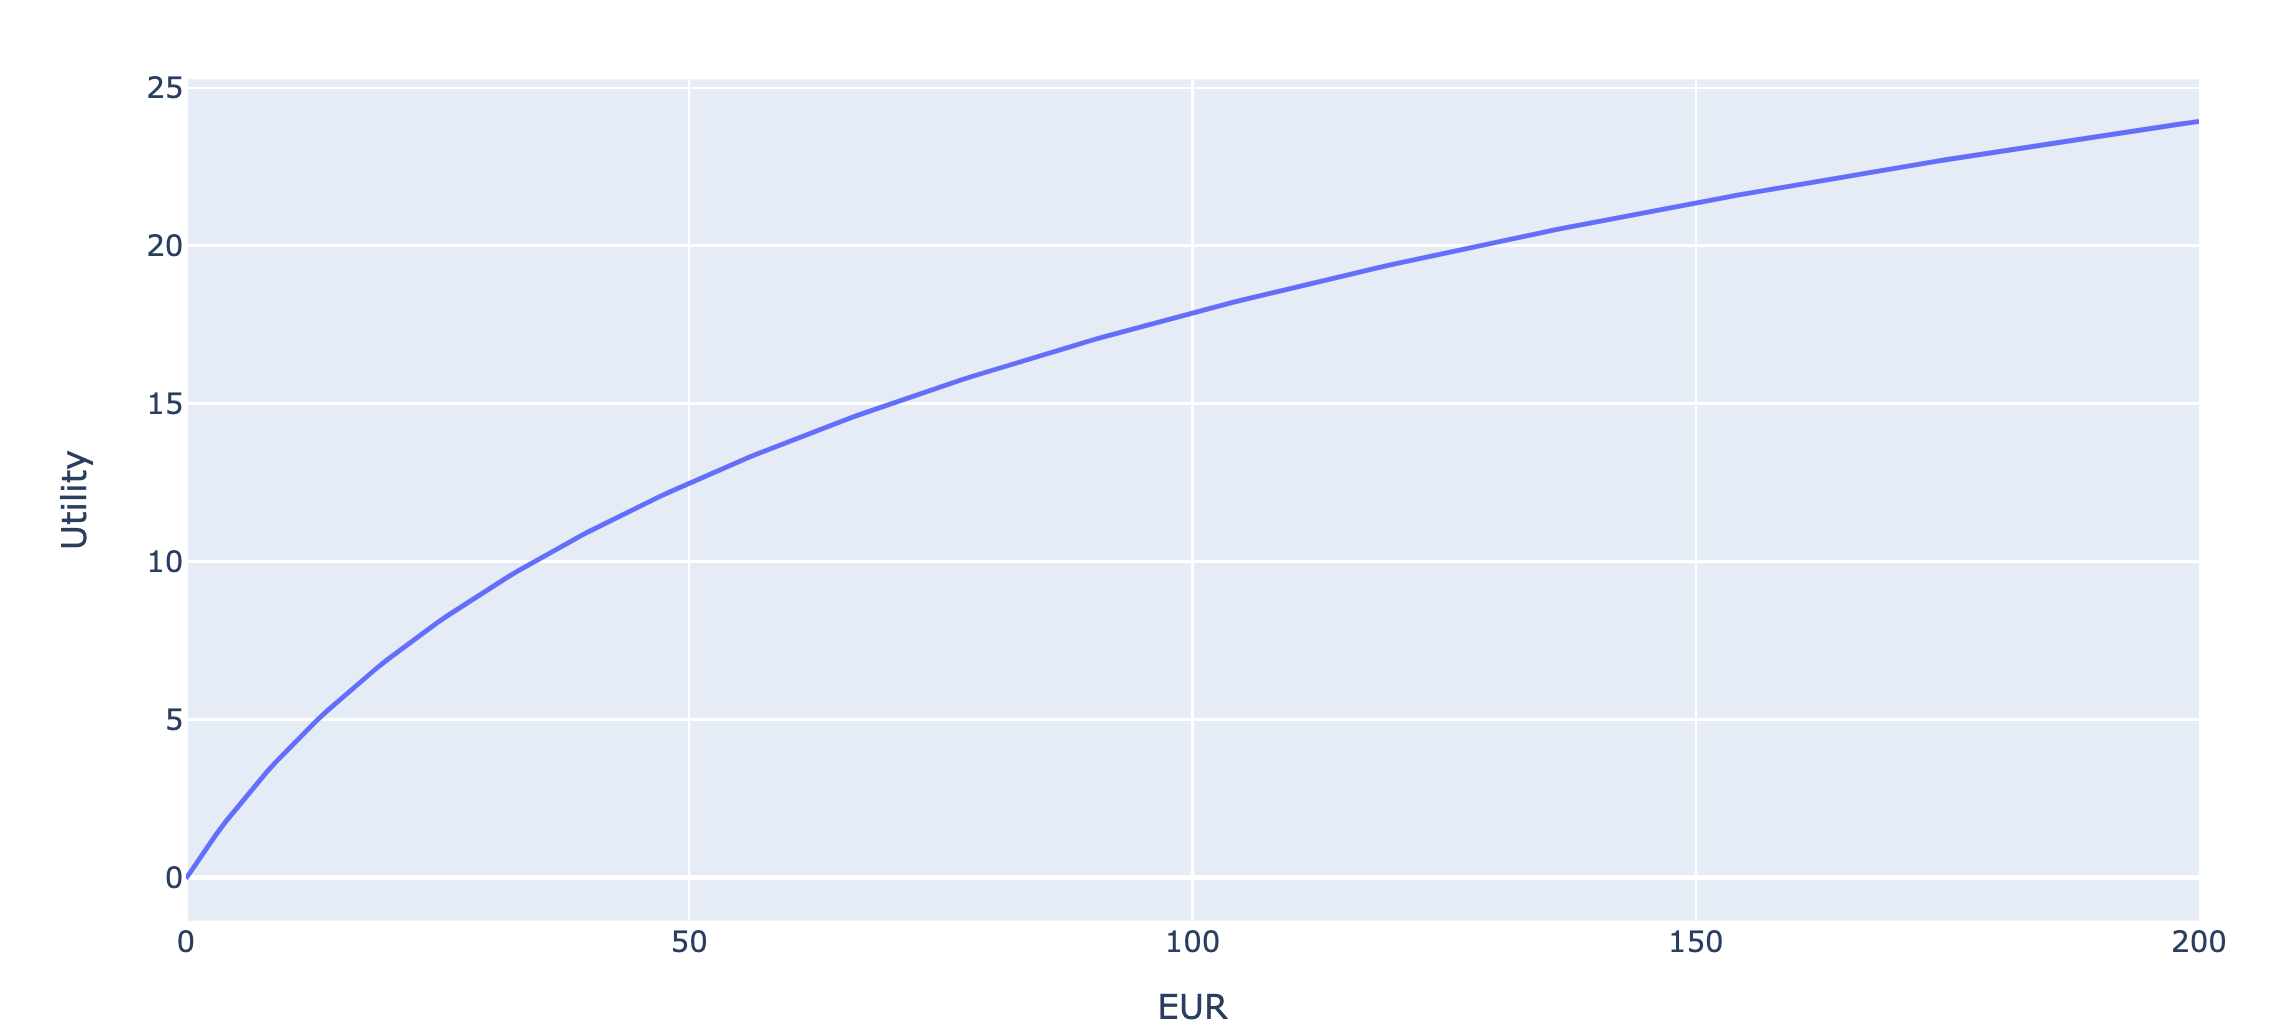
\includegraphics[scale = 0.7]{Images/UF.png}
		\caption{An example of utility function \cite{BacChi:19}.} 
		\label{fig:UF}
	\end{center}
\end{figure}



\chapter{Project valuation as stochastic decision problem}
In this chapter we develop the core idea of this thesis. The idea is to take the valuation problem as defined in ROA and solve it with SDT, while preserving the economical truths about project valuation, such as time value of money and risk aversion of investors. 

We begin by clarifying the meaning of the term project as it is used in the publications in the field of ROA. We define project valuation problem as a collection of mathematical constructs\textbf{ (?)} and identify the main limitations of this approach. 

Next, we focus on the identification of the project valuation in terms of SDT framework. We define all the relevant sets and functions to be able to talk about project valuation as a structured problem of decision making under uncertainty. 

The reminder of this chapter is reserved for the incorporation of the economical truths to the model, namely the time value of money and the risk aversion of investors. 


\section{Project valuation - problem definition}
To be able to rigorously talk about the project valuation we need to define what a \textit{project} is and what do we mean by its \textit{valuation} in ROA. The inspiration for these definitions comes from examples and used rhetoric in the ROA publications, namely \cite{Gut:09}, \cite{Vol:03} and \cite{AmrKul:98}. 

None of the books that we have studied goes in detail to define a project as a collection of mathematical constructs, as for example SDT does with MDPs. Guthrie in \cite{Gut:09} opens with a three initial examples of a project and in each chapter adds new real investment opportunity. This investment opportunity is presented in such way, that  it is clear what the project is, what are its parameters and what metric is optimized by the investor. 

In other books like Vollert's \cite{Vol:03} and Kulatilaka's \cite{AmrKul:98}  a definition of a project is also not given, rather, it is assumed that the used terms \textit{project}, \textit{capital investment} or \textit{investment opportunity} are clear. 

It is worth noting that a definition of project \textit{valuation} is also not deeply discussed in the ROA books. We feel like the term of valuation is assumed to be clear and is always represented by expected net present value (NPV), which as we discussed before is easily understandable, but not very robust metric. 

As outlined above, nothing like a clear mathematical definition of a project valuation is presented in the ROA books. However, the used rhetoric is similar and we strongly believe that the project valuation can be understood as: "An amount of value that I am able to create with actions that can be considered as a part of one project\footnote{Defined as in preliminaries}, measured by the  metric of expected net present value with a special non-axiomatic determination of the discount rate." \textbf{(???)}

Now, that the position of ROA to project valuation is clearer, we can follow with its interpretation in the SDT framework.


\section{Project valuation in the stochastic decision theory framework}
Trying to solve the project valuation task as a stochastic decision problem means first and foremost to identify all the necessary parts of the SDT framework in the ROA formulations. This in not a particularly hard task given the rather loose definition given above. 

After this identification the standard tool of SDT, dynamic programming (or potentially approximate dynamic programming), can be used to solve the valuation problem. 

Solving a valuation problem in SDT means to define it as MDP, which consists of two parts. First there are three sets: time set $\mathbf{T}$, state set $\mathbf{S}$\footnote{This global state set is a union of state set in each time $\mathbf{S_t}$} and action set $\mathbf{A}$\footnote{This global action set is a union of action set in each state $\mathbf{A_{s_t} }$}, which describe the structure of the decision making problem. The second part consists of two functions: transition probability function $p$ and reward function $r$, where $p$ is responsible for describing the stochastic evolution of the project and $r$ for informing about the value gains in each time epoch.

In the following sections we will focus on each of these five important building blocks in detail. To better illustrate each of the building blocks, and to prepare our ground for the experiment, an example concerning the valuation of a gas power plant is presented. 

\subsection{Time set}
Even though the SDT theory is capable of handling infinite time horizons and continuous time modeling, these sophisticated formats are not needed for valuation of real life projects. The time dimension of a project can be reasonably described by a discrete set with known finite horizon, which is true for two reasons. 

First is that observing new information and making impactful decisions by project's manager is not done continuously at all times but discretely after some practical time intervals. No manager changes the course of a project 10 times a day\footnote{This thesis does not focus on the individual management of the internal processes of the project. This thesis focuses on managerial decisions that modify the project in a major way.}. 

Second reason is that managers do not think about projects as ever-lasting. Potential profits after certain time threshold are neglected. This is given either by the finite-lifespan nature of the projects (gas power plant lifespan) or the extreme uncertainty in modeling of cash flows (and their equivalent is present values) in the far future. To have a good model of project's cash flow in 100 years is a wishful thinking. 


Time intervals in our model reflect the frequency of influential management meetings at which the course of the project can be changed significantly, e.g. week, month or quarterly intervals. This notion is further supported by its usage in the ROA publications. 

\begin{example}
	Monthly decision time intervals in a duration of gas power plant lifespan, say 25 years. The time set is then $\mathbf{T} = \{0,1,2,...,300\}$.
\end{example}

\subsection{State set} Defining the state set $\mathbf{S}$ in a project valuation problem means to find a list of relevant measurable parameters of both the project and its environment. A state $s \in \mathbf{S}$ is then a vector of elementary states of such individual parameters. 

The state set $\mathbf{S}$ can be constant, meaning that in each time epoch, the same parameters are measured. However, it might also be useful to think about dynamic state sets in time $\mathbf{S_t}$, $t \in \mathbf{T}$, where for some particular reasons the structure of a problem changes in time\footnote{There are more or less relevant parameters to measure.}.

It is worth noting that there are usually some elementary states that are influenceable by the managerial actions and some that are not. This classification is not reflected in our notion. 

In our models, each elementary state is understood as a random variable, which probability distribution is conditioned on the previous state and the last action taken. This probability is described with the transition probability function $p$, which is discussed in detail below. 

\begin{example}
	Relevant features for a gas power plant might be for example: price of gas, price of CO2 allowances, price of power, installed capacity of the plant, debt to be repayed or the remaining lifespan of its blocks. The first four elementary states would then be considered as uninfluenceable by our future actions, while the last three would not. 
\end{example}


\subsection{Action set}
In SDT structure the action set  $\mathbf{A}$ is usually understood as an actual set, however in the format of project valuation, we find it better to represent it as an action function, whose parameter is a  given state $s_t \in \mathbf{S_t}$ and output is a set of possible actions $\mathbf{A(s_t)}= a(s_t)$. 

The reason for this is that possible managerial actions are most of the time strictly conditioned on the current status of the project itself. Only a small subset of all possible actions might be actually taken in a given state. 

In ROA publications the term options is used to describe possible managerial actions both current and future. Even though we believe that this terminology helps with understanding that possibility of future managerial action has value, we do not embrace it in this thesis, where the standard SDT terminology is used.

The advantage of the SDT approach in contrast to ROA is that there is no theoretical  complication in adding an arbitrary amount of actions of any type (as classified in ROA by Guthrie \cite{Gut:09} for example) possibly even conditioned on one another. The only concern that needs to be reminded is that of computational complexity, where large number of possible managerial actions decrease the ability to compute the valuation in practice. 

\begin{example}
	Actions in gas power plant project might be to: build new block of the plant, run the plant if it has some installed capacity, mothball or sell the power plant for salvage value. 
\end{example} 

We believe that this example clearly shows the dependency of possible actions on given state and why is it thus better to use the function notion from now on. 

With the definition of action set, now function, we have defined the general structure of a project, boundaries within which the project will evolve. Now we will study the rules that guide the evolution and metrics that measure the value created. 

\subsection{Transition probability function}
Given the nature of projects, the evolution from one state to another is stochastic. In this thesis we want to model the project as MDP and thus the probability distribution of the next state, described by so called transition probability function, is conditioned only on the previous state and the last action taken. In mathematical notation: 
\begin{equation}
	p(s_t|a_{t-1}, s_{t-1}).
\end{equation}

The probabilities in this thesis are understood as both discrete probabilities and probability distributions in case of continuous variables. Furthermore, as we will model each elementary state by a different distribution we need to be able to compute the overall probability of the future state given the elementary distributions. 

To make things simple, we assume individual elementary states to be represented by independent variables and thus the probability (or probability distribution) of a next state is a product of the elementary probabilities\footnote{Combination of discrete and continuous variable as elementary states results in continuous global variable (and thus probability distribution).}: 

\begin{equation}
	p(s_t|a_t, s_{t-1})=\prod_{i}p(s_t^i|a_t, s_{t-1}), 
\end{equation}
where $s_t^i$ is the i-th elementary state of $s_t$.

\begin{remark}
	It is possible that some elementary states are fully determined by the managerial action $a_t$. Such corner case does not create a problem for the probabilistic notion above, the new elementary state $s_t^i$ is realized with probability $p(s_t^i|a_t, s_{t-1})=1$.
\end{remark}

It is clear that in the majority of real-life projects, determining, or estimating, this transition probability function is a very hard, but crucial task. Decisions will be made based on its values increasing or decreasing the value of a project. 

The approach of ROA authors to modeling of these probabilities varies a lot. Some authors like Guthrie \cite{Gut:09}, or Amram \cite{AmrKul:98} use the arbitrage principle to determine the probabilities of their binomial models. Some authors, like Kulatilaka \cite{KulTri:94}, use the principle of insufficient reasons\footnote{Even though they do not call it that way.}, where they assign 50\% probability to movements in both directions of their binomial models. Some authors, like \cite{Gut:09} and \cite{Vol:03}, go also deeper in statistical modeling of the probabilities. 

Some details of how does SDT approach the estimation of $p(\cdot)$ will be discussed later in section \ref{sec:probability}, however we must note that correct estimation of these probabilities is not the focus of this thesis.


\subsection{Reward function}
The final part of modeling the project valuation as MDP is the reward function. Its purpose is to assign a numerical value to the state realization given the previous state and last managerial action, mathematically: 

\begin{equation}
	r(s_t|s_{t-1}, a_{t-1}).
\end{equation}

As discussed in preliminaries, the notion of ``value`` is complicated. In our case of project valuation, the first approximation of the entity that is to be maximized is the free cash flow (FCF). FCF usually consists of expenses, which are a result of immediate managerial actions, and income, which tends to be a result of the environment (supply and demand for manufactured products or services) conditioned on a previous action or action sequence. 

Usually, the goal of MDP is to find a strategy, which maximizes the expected reward. However, as economical theory guides us, there is a clear preference in having money now instead of later (time value of money) and that investors do not value uncertain rewards the same as their expected values (risk aversion of investors). Both of these phenomena lead us to build a generalization of the reward function, that reflects them and its optimization defines the optimal strategy in projects defined as MDPs.

The incorporation details of these phenomena will be discussed deeply in the following sections \ref{sec:time_value_of_money} and \ref{sec:risk_aversion}. For now, lets declare that the generalized reward function will be based on FCF, adjusted for individual risk preferences and borrowing and risk-free investment opportunities of the investor.

\begin{example}
	Reward function of a gas power plant is driven by its ability to make money by transforming the gas and CO2 allowances into the electrical power. The initial expenses for building the individual blocks result in extreme negative rewards (driven by action of building), while the profits are made as a multiple of installed capacity and the difference of input costs plus static costs and the revenue from selling the electricity (conditioned on action of running the plant).
\end{example}

\bigskip

This paragraph concludes the basic identification of sets required by the SDT framework. In the next section, we will focus on the solution to the project valuation problem in detail. We will discuss the sources of transition probability function, the actual incorporation of time value of money and the risk aversion of investors into the model. 

\section{Solution of the project valuation as SDT problem}
In the previous chapter, we focused on the basic structure of a project valuation understood as MDP. In this chapter we go deeper and we focus on the details of the actual solution of such valuation problem. 

We begin this section by looking in detail at the estimation of the transition probability function $p$. We outline, how the SDT can not only incorporate the ideas of ROA, but also help with more advanced estimation techniques. 

Then, we pursue with incorporation of the economical truths - time value of money and risk aversion of investors in a form of utility maximization principle and the notion of PCE. We focus on implementation details with accent on applicability by real-life managers. 

Finally, the last part of this section addresses the computational complexity problems of classical dynamic programming, proposing an algorithm from the ADP class, identified as the best fit for a project-valuation-style MDPs. 


\subsection{Probability}\label{sec:probability}
In this thesis we focus on real-life projects. Such projects are from their nature stochastic and except for some edge cases, the laws guiding the evolution of the relevant parameters are unknown and complex. Our search for the optimal strategy is based on the assumption that we have some model estimating the future paths of the project states and we act as if this model was the reality. In our case the model of this evolution is materialized in a form of transition probability function $p$, where for example one of the assumptions is the Markovian property of the states. 

There are many ways how to model $p$. Let's discuss the techniques used in ROA publications and how they can be translated into SDT terminology. Furthermore, lets also outline the more advanced techniques that SDT can offer in this section. 


\paragraph{Risk neutral probabilities}
The idea of risk neutral probabilities is the major modeling force in the ROA publications. We observe two levels of its usage, both of which are based on the non-existence of arbitrage. 

First, simpler approach, used by \cite{Ryu:17} or \cite{DamZro:19}, adjusts only for the time value of money represented by the risk-free rate $r_f$, where the probability of up move is computed as:
\begin{equation}
	\pi_u = \frac{Xr_f-X_d}{X_u-X_d}, 
\end{equation}
where $X, X_u, X_d$ are the values of the asset now, after one up move and after one down move. This equation represents the idea that the probability of up move of an asset is such that its expected appreciation is only the risk-free interest rate. 

The more complex equation, adjusting also for the specificity of the risk of the field, wee invest in, called risk-premium comes from the capital asset pricing model (CAPM). This model is used by the frequently mentioned Guthrie in \cite{Gut:09}, but also in other publications, like \cite{LunDid:17}.

This techniques is used for binomial models, but it is easy to imagine its usage for its limit case which is a variable with the Poisson distribution. 

\paragraph{Insufficient reasons}
The second widely observed modeling style in ROA publications, observed again mostly with the binomial models, is to assign 50\% to both up and down move. This technique can be used on different levels of the model, as the final model \cite{AmrTri:94} or for example as a helping distribution modeling a particular non-final distribution as in \cite{Gut:09}.

It needs to be emphasized that the ROA authors do not use this terminology themselves. 

\paragraph{More complex models}
In more mathematical publications we observe more complex models of the future state outcomes. For example the normal process with dynamic parameters \cite{BenWhi:17} or \cite{AlsWan:20}, mean-reverting process with Poisson jumps \cite{SchRob:19} or the modeling by a general \^{I}to process \cite{Vis:18}. 

It seems that these models come from authors with more mathematical than economic background and their unifying feature is the rigorous usage of random variables and continuous distributions. 


\paragraph{SDT interpretation}
Now we would like to discuss the interpretation of the ROA techniques in SDT. The notion of risk-neutral probabilities can be approached with the framework of `expert knowledge`` where the first expert is the one (usually the economist using the CAPM formula) who determines the individual variables like the risk-premium, or expected market growth. In accordance with the philosophy of experts, the second expert is the market behaving by the non-arbitrage principle, giving us the equations for risk-neutral probabilities. 

The term of insufficient reasons comes from the SDT itself and thus it was already interpreted above. 

The class of more advanced approach that we have discussed above is easily covered with the SDT too because of its structure. The outputs in terms of distributions, coming either from the data or again the ``expert knowledge`` are easily incorporated into the SDT framework as prior (static or dynamic) probabilities.   

\paragraph{SDT innovation}
The portfolio of SDT estimation techniques is much wider than it was discussed so far. Because probability estimation is not the main focus of this thesis, we will only outline two of the most interesting techniques. 

First is the Bayesian modeling, where each time new data are being observed, our probability model is updated by the Bayesian formula. This very influential modeling technique in SDT was not seen in the ROA publications, even though there is certainly a space for it. 

The second modeling strategy that we want to talk about is the consistent way of information fusion from different sources. This niche part of the SDT, lead by Karny \cite{Kar:20}, allows for incorporation of multiple sources of prior probabilities, for example multiple experts, data sources, and more \textbf{(?).}

\paragraph{Summary}
To conclude, we advice to use one of two approaches to the problem of $p$ estimation. First, when a lot of information about the project is known, we have a strong case for the parameters behaving according to our smooth distributions, and we believe the market to compactly reflect the expert knowledge, we prefer Bayesian updated risk-neutral probabilities. 

On the other hand, if the project is truly innovative and there is very little data to base our model on, we prefer to use a combination of expert knowledge and principle of insufficient reasons. 

In the end, we leave the decision of the actual modeling to the framework user, where we express the sympathy for simple models, where more ``unclear`` models in spite of their better precision, might not be accepted by the board making the investment decision. Clearly, we do not advice to use advanced SDT modeling techniques like probability distribution fusion. 



\subsection{Time value of money}\label{sec:time_value_of_money}
As outlined in preliminaries, money does not have the same value through time. This economical truth is one of the most important ones in project valuation and capital budgeting. The approach of the economical theory to this problem is to exponentially discount the future cash with so called risk-free interest rate. 

In the studied ROA publications, the problem of different borrowing and risk-free investment rate is not addressed. The ROA publications assume that the investor is able to borrow at the risk-free interest rate, which is in reality not the case. 

In our modeling, the first approximation of the optimized entity was the expected sum of future cash flows. Now, we can present the second approximation of the optimized entity, which is somehow new for both the ROA and SDT\footnote{SDT theory uses exponential discounting for example in models with infinite time sets, however we have not been able to find a study of discounting conditioned on a state\textbf{(?)}.} world. 

This newly defined entity is called present cash equivalent (PCE) and it represents the amount of money that an investor is logically indifferent to having instead of a vector of future cash flows. As argued in preliminaries, this value is unique and for natural borrowing and risk-free rates always defined. 

The second approximation of the MDP's optimized entity is thus the expected present cash equivalent of the free cash flow vector of the project, mathematically: 

\begin{equation}
V(s_{t-1}) = \max_{a_{t-1} \in \mathbf{A_{s_{t-1}}}}\sum_{s_t \in \mathbf{S_t}} p(s_t|a_t, s_{t-1}) PCE_{t-1}\left(r(s_t|a_t, s_{t-1})+V(s_t), s_{t-1}^b\right),
\end{equation}
where $s_{t-1}^b$ is the project's balance state in time $t-1$. 


\begin{remark}
	It needs to be clarified that if we want to embrace the notion of ROA publications, where we assume the simple discounting of the FCF, we are able to do it with this framework too. This notion is only a corner case of our framework, where the borrowing rate is equal to the risk-free rate. 
\end{remark}


\subsection{Risk aversion of investors}\label{sec:risk_aversion}
As discussed above, the nature of real-life projects is stochastic. The uncertain evolution of states results in the uncertain FCFs defined by the function $r$, which has implications for the decision making of investors. 

As discussed in the preliminaries, section \ref{sec:risk_aversion_preliminaries}, the majority of investors is risk averse, meaning that they tend to value uncertain gains lower than is their expected value. 

We believe that this characteristic of investors is important to consider in the valuation of a project. Fortunately, the SDT theory already has a framework for coping with such skewness in reward perception called utility theory. 

The third and final approximation of the optimized entity by the Bellman equation is thus the expected utility of the present cash equivalent of individual cash flows. The third and final update of the original Bellman equation can be thus described as: 

\begin{equation}\label{eq:third_approximation}
	V(s_{t-1}) = \max_{a_{t-1} \in \mathbf{A_{s_{t-1}}}}\sum_{s_t \in \mathbf{S_t}} p(s_t|a_t, s_{t-1}) \mu\left(PCE_{t-1}\left(r(s_t|a_t, s_{t-1})+V(s_t), s_{t-1}^d\right)\right),
\end{equation}


\begin{remark}
	Even though there are consistent methods for obtaining the utility function of the individual investors, it might be hard to get individual investor on board with the idea of utility\footnote{Investor might not have a time to answer the utility questionnaire as suggested by \cite{BacChi:19}.}. This does not present a fundamental problem for our valuation technique, because we can always use the utility of the risk-neutral investor, which is unique and its usage supported by the lack of bias against uncertain outcomes. 
\end{remark}



\subsection{Approximate dynamic programming}


As mentioned in the previous sections of this thesis, the classic DP algorithm can be used for computing the optimal strategy MDP's only with rather small cardinalities of the $\mathbf{A}$, $\mathbf{S}$ and $\mathbf{T}$ sets. This known DP problem is in literature addressed as ``three curses of dimensionality`` \cite{Pow:11}.

Real-life projects, interpreted as MDPs are usually rather complex and hardly-ever fulfill this condition. For example, when even one measured parameter is modeled to come from a continuous distribution, the DP algorithm brakes down not only from the limitation of the actual computational complexity, but also theoretically. 

It might be clear from the rhetoric of this thesis, that our goal is to use the developed valuation technique in practice. That is why we want to address this problem with the goal to make the solvable class of project valuation problems as large as possible. And we do so with the approximate dynamic programming (ADP) approach. 

From all the possible ADP techniques, we have chosen the value iteration with parameter model approximation for two main reasons, both of which originate in the fundamental characteristics of projects.

First is that the real-life projects tend to have large state spaces (even uncountable), while on the other hand the action set is usually limited. We cannot ask a manager to make a choice between 10 000 actions for example. This supports the choice of value iteration over a policy iteration class of ADP. 

Second is that we usually have a good intuition of what exactly in the given states ``makes money`` and we are able to identify and cluster the important parameters. This allows us to build a reasonable basis function set, which should produce a good approximation of the value function.


It needs to be clarified, that even though we believe that our approach is generally the best, regarding the mathematical complexity, its precision and clarity, there might be better ADP algorithms for individual projects the reader intends to value. 

\subsection{Summary}
This subsection summarizes the core idea of this thesis. 

Firstly we have presented the interpretation of the project valuation problem as a MDP. We have  defined all its important parts in detail and offered examples for clarity.

Secondly, we have adjusted the MDP theory to respect the economical truths with the notion of PCE respecting the time value of money and utility function interpretation of the investors' risk aversion.

Lastly, we have advised the best ADP algorithm that copes with the problems of computational complexity of the usual DP solving algorithm for non-trivial projects. 






\chapter{Valuation of facilities with simple I/O process}\label{chapter:Experiment}
In the previous chapter, we have presented an algorithmic approach to a project valuation based on the SDT framework and its ideas. Now we want to illustrate the actual usage of this algorithmic approach on a chosen class of projects. 

We have chosen the class of projects that can be labeled as an investment in facilities with a simple I/O process and further managerial guidance. This class is characterized by a large outflow of money at the beginning used for building the facility (or its first functional part) and a small but long-term positive future revenue driven by the difference in the price of inputs and outputs of the facility and the further managerial decisions. 

This class choice is supported by its appropriate level of complexity, where it allows to demonstrate the power of the new algorithm while at the same time not being too complicated. It is also a type of project that is substantially represented in the world of capital investment. 

We could write this whole chapter using a general description of the chosen project class; however we believe that using only one specific representative will result in a clearer picture of the situation. 

Our choice of the representative - an investment into a gas power plant - is based on three grounds. First, there is certainly an influence of Guthrie's example of a similar valuation problem \cite{Gut:09}. Second, as we will see, this valuation problem has reasonable dimensions that allow for a good presentation of the valuation algorithm. Lastly, the author of this thesis has legitimate domain knowledge based on his short but intensive work experience in the field of power trading. 

In the first part of this chapter, we will describe the valuation problem with the utmost precision. 

In the second part, we will compare the PCEs of three baseline operational strategies and the optimal one derived from the valuation algorithm. Furthermore we will study the influence of the increased volatility of prices on the final valuation. From what we have learned about the value of options, the project's value should increase together with the volatility increase. 

It needs to be emphasized that the aim of this experiment is to present the valuation algorithm, observe and describe its possible shortcoming and support its viability, not to prove any other theorems or ideas about project valuation.


\section{General settings of the experiment}
First, let us clarify what we mean by the phrase \textit{investment in the gas power plant}. We are positioning ourselves in the role of an investment analyst of a large utility company\footnote{Companies that generate electric power usually provide also gas, water, sewage or other basic services.} whose task is to evaluate the value of building and managing a new gas power plant. 

For simplicity, we are considering building only one or two 200MW blocks, the lifespan of which ends 25 years from now, disregarding the time they were built  \cite{Car:12}. We assume that each block's price is 65M EUR, which is a rough estimate based on \cite{Bre:10}. 

We model the power plant to be managed in a monthly pattern. Its power is being sold by monthly contracts at the beginning of each month, when the needed gas and CO2 inputs are also modelled to be purchased. This results in certain free cash flows that are assumed to be obtained immediately after taking one of the allowed actions. As was indicated earlier in this thesis, we do not want to go deep into the plant management and its internal processes. 

Regarding the project's financing, we assume that the majority of the initial payment will be made by a flexible loan\footnote{An ideally flexible loan where we can repay any amount at any time.} with an interest rate of 6\%. We define the risk-free interest rate as 2\%. The reality of having non-zero initial funds is reflected in the existence of the corresponding elementary state. 

Now that we have clarified the project that we want to value, we can proceed with precise definitions of the MDP parts. 


\subsection{Time set}
As outlined in the introduction of this chapter, we assume that the lifespan of a gas power plant is 25 years, and it is managed on a monthly basis, thus the time set is defined as: 
\begin{equation}
\mathbf{T} = \{0,...300\},
\end{equation}
where the epoch $300$ is understood as the final epoch, where no actions can be made, and no FCF can be obtained. 


\subsection{State set} 
The state set needs to consist of the smallest number of relevant parameters that enable us to model the process of building and running the power plant and capturing the FCF and its derived metrics of the project. 

As such, we identify five elementary states as parameters describing:
\begin{itemize}
	\item the price of gas- $s^1$
	\item the price of CO2 allowances - $s^2$
	\item the price of power  - $s^3$
	\item number of blocks built - $s^4$
	\item cash balance of the project (models the debt) - $s^5$
\end{itemize}
in the start of each time epoch (month).

The states of the state set are defined as having a constant length, since there is no significant change in relevant parameters through the project. 

Mathematically the state set $\mathbf{S}$ is defined as: 
\begin{equation}
	\mathbf{S} = \{(s^1,\dots,s^5)|s^i \in \mathbf{S^i} \ i \in(1,...,5))\}, 
\end{equation}
where $\mathbf{S^i}$ represents the limitation of the individual elementary states. These limitations will be in detail discussed now. 

For the states representing prices, $s^i, i \in \{1,2,3\}$, we define: 
\begin{equation}
	\mathbf{S^i} = \mathbb{R}_{0}^+.
\end{equation}

The next elementary state, $s^4$, represents the number of blocks built, simply:
\begin{equation}
\mathbf{S^4} =  \{0,1,2\},
\end{equation}

The final elementary state, representing the financial balance of our project is then allowed to have any real value:
\begin{equation}
	\mathbf{S^5} = \mathbb{R}.
\end{equation}

These definitions represent the problem structure, the boundaries within which the simulation of initial investment and further managerial actions will take place. 


\subsection{Action function}
In this experiment, we consider four managerial actions. They could be understood as two-dimensional, where the first dimension represents the act of running the installed capacity of the plant (if one exists), whereas the second manages the action of building new blocks. However, we have decided on a one-dimensional form with actions encoded as: 
\begin{itemize}
	\item 0 - do not change the current state of the project,
	\item 1 - run the existing installed capacity,
	\item 2 - run the existing capacity and build a new 200MW block,
	\item 3 - build a new 200MW block.
\end{itemize}

As discussed earlier in this thesis, certain actions are available only in certain states. The state that determines what actions are possible is exclusively the elementary state $s^4$ describing the number of blocks built. 

In the following list, we express the possible action set in possible elementary states $s^4$ with a short explanation.

\begin{itemize}
	\item $a(s^4=0) = \{0,3\}$ when nothing is built, we can build the first block or do nothing and wait. 
	\item $a(s^4=1) = \{0, 1, 2, 3\}$ when only one block is built, all actions are possible. 
	\item $a(s^5=2) = \{0,1\}$ when two blocks are built, the building actions are not possible. 
\end{itemize}


\subsection{Transition probability function} 
The best way to describe the model of evolution from one state to another is to assume the independence of individual elementary states, which allows computing the probability of state transformation as a product of transition probabilities of the individual states: 
\begin{equation}
	p(s_{t+1}|s_t,a_t)= \prod_{i = 1}^{5} p(s_{t+1}^i|s_t^i,a_t^i).
\end{equation}

In our example, there are five elementary states, where the ones representing prices of gas, CO2 allowances and power are modeled in the same way. The other two elementary states are deterministic but differ in the dependency on the previous state and action. Let's now describe the evolution of the individual elementary states in detail.

\paragraph{Commodity prices}
The prices of gas, CO2 and power are modeled by the geometric Brownian motion, the model used in the BSM model and other publications like \cite{Vol:03}.

The probability of the next elementary state is thus conditioned only on the value of the previous state as: 
\begin{equation}
p(s_{t+1}^i|s_t^i) = s_t^i\cdot e^{(\mu -\frac{\sigma_i^2}{2})dt+\sigma_i W_{dt}}
\end{equation}
for $i \in \{1, 2, 3\}$, where $dt$ represents a time fraction in years, for us $1/12$ and $W_t$ is a Wiener process with probability density function defined as: 
\begin{equation}
p_{W_t} = \frac{1}{\sqrt{2\pi t}}e^{\frac{-x^2}{2t}}.
\end{equation}


 To be able to model the prices, we need to supply the variances $\sigma_i$ and the initial values $s_0^i$ for all $i \in \{1,2,3\}$.
 
 The initial prices that we use are inspired by the real prices of commodities that are being traded on the Intercontinental exchange (ICE). In this thesis, we would like to avoid going into the details of plant efficiency and unit transformation, thus we present the initial prices as illustrative and already transformed to EUR per MWh produced.
 
 Similarly, the values of individual commodity volatilities are inspired by our experience with the ICE and the realization of commodity prices in recent years. However, they still remain only illustrative. 
 
 In table \ref{Table:init_values} we can see the chosen initial prices and two triplets of volatilities, which are presented due to a second goal of this experiment, determining the influence of volatility on the value of a gas power plant project. The second triplet is chosen simply as a 20\% increase of the first. 
 
 \begin{center}
 	 		\label{Table:init_values}
 	\begin{tabular}{|l |r |r |r|} 
 		\hline
 	    &	Initial price [EUR] & Volatility 1 & Volatility 2 \\  
 		\hline
 		Gas & 25 & 0.12 & 0.144 \\ 
 		\hline
 		CO2  & 10 & 0.10 & 0.12 \\
 		\hline
 		Power & 37 & 0.15 & 0.18 \\
 		\hline

 	\end{tabular}
 \end{center}
 
\paragraph{Installed capacity}
The evolution of elementary state $s^4$ representing the number of blocks built is deterministic and conditioned on the previous action. If the chosen action is $a = 2$ or $a=3$, representing building a new block, then the elementary state of the number of blocks increases by 1 with probability 1. If chose action is $a=0$ or $a=1$ this elementary state is not changed with probability 1, mathematically: 
\begin{equation}
p(s^4_{t+1}=y|s^4_t = x, a_t) =
\left\{
\begin{array}{ll}
1  & \mbox{if } x = y \land a_t \in \{0,1\}  \\
1 & \mbox{if } x+1 = y \land a_t \in \{2,3\} \\
0 & \mbox{otherwise} 
\end{array}
\right.
\end{equation}

\paragraph{Balance}
The last model that needs to be discussed is the one representing the financial balance of the project. This state simulates the actual cash balance driven by actions of a "responsible manager", the assumptions of ideal loans\footnote{With the availability to repay any amount of money at any time.} and the possible risk-free investment with constant interest rate. 

Based on two types of monthly interest rates, the one for which the investor can borrow in a bank $r_b=\sqrt[12]{0.06}$ \footnote{We assume the yearly borrowing interest rate of 0.06\%} and the one of risk-free interest rate $r_r=\sqrt[12]{0.02}$, we define the evolution of $s^5$ as: 
\begin{equation}
p(s^5_{t+1}=y|s_t, a_t,  s_t^5=x) =
\left\{
\begin{array}{ll}
1  & \mbox{if } y = RM(FCF(s_t, a_t)+x, r_b, r_r)\\
0 & \mbox{otherwise,} 
\end{array}
\right.
\end{equation}
which means that this elementary state is deterministic and its value $s^5_{t+1}$ is computed as a result of responsible managerial actions with the previous balance $x$ adjusted for the FCF obtained in the previous state $s_t$. 

The actual computation of $FCF(s_t,a_t)$ will be revealed in the next section, whereas the $RM(\cdot,r_b,r_r)$ function can be found in preliminaries. The model allows for easy interpretation of non-zero initial balance, however in our experiment we define $s^5_0=0$.  



\subsection{Reward function}
The FCF model in our example, and actually in all projects in the class of facilities with simple I/O process, is fairly straightforward.

First, we account for the fixed price of maintenance $C_m$, which in our case is $C_m=6$ EUR/MW of installed capacity for each hour. 

Then, conditioned on the action of running the facility, we account for commodity input costs (here gas and CO2). Finally, we add the profit from selling our product on the market and the computation for FCF is complete. 

The mathematical expression of the sentences above can be presented as:
 
 \begin{equation}\label{eq:fcf_function}
  	FCF(s_t,a_t) =s_t^4 \cdot \Big[-C_m + I_{\{1,2\}}(a_t)\cdot (s_t^3 - s^1_t - s_t^2)\Big]\cdot 200 \cdot h_m
 \end{equation}
 where $h_m=720$ is a constant representing approximation of hours in month, not accounting for the changes in month lengths. 

\begin{remark}
	As discussed earlier, the optimal strategy is not being optimized for the expected cumulative FCF, but rather each action optimizes the expected utility of the present cash equivalent in the current state. 
\end{remark}

 
 \section{Approximate dynamic programming}
 
 In preliminaries we have discussed the algorithm for modelling the value function with some general function $v_f(s)=f(\phi_i(s))$. Now, as we have defined our problem, we are able to outline the specific model for our case. 
 
 Based on the initial observations of state-utility pairs comming from the performed simulation (see algorithm \ref{alg:VFapp} step 10 and figure \ref{fig:PW_linear}) and the intuition that the FCF function \ref{eq:fcf_function} gives us, we have decided to model the value function with a model of three picewise linear models with one breaking point $x_{i,t}, y_{i,t}$: 
 
\begin{equation}\label{eq:VFmodel}
	v_t(s) = \sum_{i} I_{i}(s^4) PW(s^3-s^2-s^1, k_{i,t}^1, k_{i,t}^2, x_{i,t}, y_{i,t}), 
\end{equation}
where $I_i$ is an identificator function of installed capacity $s^4$, and $k_{i,t}^1$,  $k_{i,t}^2$ the slopes of the piecewise linear function model $PW$. For a better illustration, we present an example of such model fitted to the real data. figure \ref{fig:PW_linear}.


\begin{figure}[htb]
	\begin{center}
		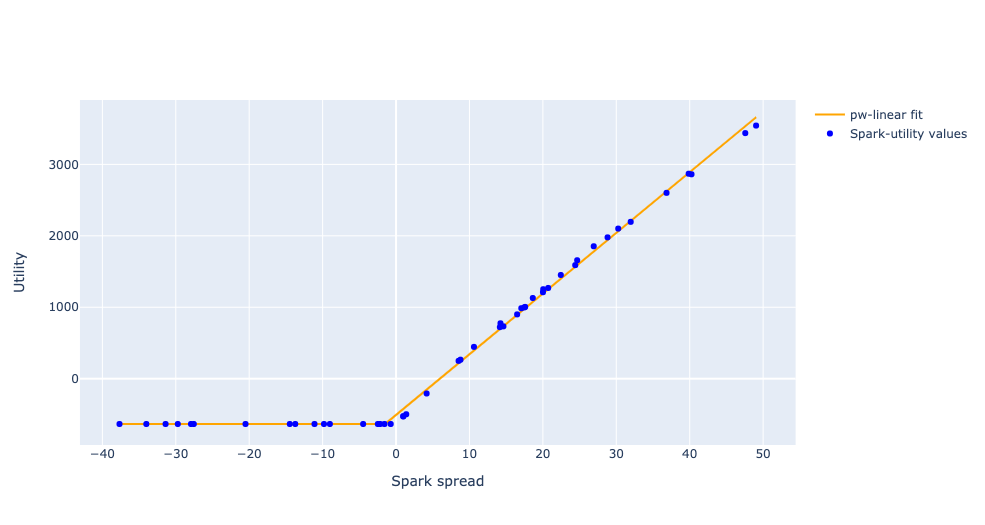
\includegraphics[scale = 0.7]{Images/pw_linear_example.png}
		\caption{Example of a pw linear fit.} 
		\label{fig:PW_linear}
	\end{center}
\end{figure}
 
 
This model effectivelly reflects only two variables, the installed capacity of the power plant, reflected by the choice of three models and generalized "spark spread" $s_t^3-s_t^2-s_t^1$ which reflects how much money is being made by running the plant with the current costs of inputs and the market price of power. 

The value function in each time epoch $t$ can thus can be represented by tvelwe variables $k_{i,t}^1, k_{i,t}^2, x_{i,t}, y_{i,t}$ for $i \in \{1,2,3\}. $

To determine these parameters for our example, we will use the ADP algorithm of value iteration, which we describe in general and then we will discuss the details of individual steps. 

\begin{algorithm}
	\caption{ADP value iteration algorithm}\label{alg:VFapp}
	\begin{algorithmic}[1]
		\Require{$v_{300}(s)$}
		\State Prepare empty list $L$ for vf model parameters
		\For{ t $\in (299,298,...0)$} \Comment{Backward epoch induction}
			\State Prepare state sample $S_t$ \Comment{See paragraph state sampling}
			\State Declare empty list of state utility pairs $l$
				\For{$s \in S_t$}
					\For{$a \in a(s)$} \Comment{All allowed actions in given state}
						\State\parbox[t]{.5\linewidth}{Evaluate the expected utility of an action $a $, $u_a$ given $v_{t+1}$ approximation} \Comment{See expected utility paragraph}
					\EndFor
					\State Determine $\max_{a \in a(s)}u_a = u$.
					\State Save $(s,u)$ pair in a list $l$.
				\EndFor
			\State Fit the $(s,u)$ pairs from $l$ to the model described by equation \ref{eq:VFmodel}
			\State Save the fit parameters  $k_{i,t}^1, k_{i,t}^2, x_{i,t}, y_{i,t}$ for all $i \in \{1,2,3\}$ in a list $L$
		\EndFor
		\State	\Return{$L$}
	\end{algorithmic}
\end{algorithm}

\paragraph{Last VF}
For the consistency in notation, there is a need for definition of the value function in the last epoch, where no action is possible anymore. Since the value function represents the metric of expected reward in the future, its value is 0. In our case the $v_{300}$ is represented by the same model shown in equation \ref{eq:VFmodel} with all parameters equal to 0. 

\paragraph{State sampling}
In the third step of our algorihtm, we define a state sample. This state sample serves the purpose to reasonably cover the uncountable state space with finite number of values. In this thesis, we create the sample by making samples of individual elementary states which are then randomly put together creating a random realization of a global state. 

In the following table, we describe the distributions out of which the elementary realizations are taken. 
\begin{center}
	\label{Table:sample_values}
	\begin{tabular}{|l |m{4cm}|} 
		\hline
		Elementary state&	Distribution  \\  
		\hline
		Gas price & Uniform(0,30) \\ 
		\hline
		CO2 price  & Uniform(0,40)  \\
		\hline
		Power price & Uniform(10,80)\\
		\hline	
		Number of blocks & $p(s^4=0)=0.3$ \newline  $p(s^4=1)=0.35$ \newline $p(s^4=2)=0.35$ \\
		\hline	
		Balance& Uniform(-60M, 60M), \\
		\hline	
	\end{tabular}
\end{center}

All the random variables are generated by python llibrary numpy and the sample size was chosen as $|S_t|=100$.

\paragraph{Expected utility}
In step 7 of the algorithm \ref{alg:VFapp}, we want to assign individual action $a$ in state $s$ the expected utility. This assignment is made with the help of the equation \ref{eq:third_approximation}, respective its part: 
\begin{equation}\label{eq:exp_util}
	\int_{s_t \in \mathbf{S_t}} p(s_t|a_t, s_{t-1}) \mu\left(PCE_{t-1}\left(r(s_t|a_t, s_{t-1})+V(s_t), s_{t-1}^d\right)\right) d s_t,
\end{equation}
which was adjusted for our continuous case, changing the sum for an integration. 

To compute this expression we use a simple numerical integration technique. Based on the state in which we are in $s_t$ and the transition probability function $p(s)$ defined above we simulate chosen number of state evolutions, here $n=100$. Then the results of the numerical integration is the average of the individual utilities of PCEs of the realizations $s_{t+1}$..


\paragraph{Model fitting}
In step 10 of our ADP algorithm the data from list $l$ are being fitted by the model described by the equation \ref{eq:VFmodel}. We do this in reality by fitting three individual subsets, one for each of the plant states, by the pw linear function with one breaking point. The individual fits are done with the help of python library lmfit which is using the least square evaluation metric. 


\section{Optimal strategy performance}
Now, that we have the estimation of the value funciton in our hands, we are able to value the project. The only thing that we need to do, is to insert the chosen initial state $s_{init} = (25,10,37,0,0)$ defined above by parts into the model of $v_0(s_{init})$, which gives us the result of 349M EUR. 

Now, we want to verify the sensibility of this result by simulation of the actuall decision making process and comparing it with some baseline strategies. Let us first define these strategies and then the simulation algorithm according to which we will compare them to the optimal strategy. 

\paragraph{Baseline strategies} 
\begin{itemize}
	\item Strategy $B_1$ builds two blocks of the powerplant in time epoch 0 and 1 and then runs them no matter all the other factors.
	\item Strategy $B_2$ builds two blocks of the power plant similarly to strategy $B_1$ but it runs the plant, only if the prices are favorable, meaning $s_t^3-s_t^2-s_t^1-C_m>0$. 
	\item Strategy $B_3$ does not build the blocks righ away, but waits for more favorable market states than the $s_{init}$ provides. It builds new block only when the generalized spark price rises above arbitrarily chosen amount of 40 EUR ($s_t^3-s_t^2-s_t^1-C_m>40$). The rule for running the installeed capacity remains the same as for the strategy $B_2$
\end{itemize}

\paragraph{Simulation algorithm}
In this paragraph we will describe the simulation of the decision making upon which we compare the performance of our optimal strategy and the baseline strategies $B_i$ $i \in \{1,2,3\}$.


\begin{algorithm}
	\caption{Strategy performance algorithm}\label{alg:Simulation}
	\begin{algorithmic}[1]
		\Require{Strategy $B$, $r_r$, $r_b$} \Comment {Baseline  vf approximation based}
		\State Define intitial state $s_0 = (25,10,37,0,0)$
		\For{ t $\in \{0,1,...299\}$} 
			\State Determine action $a_t$ in state $s_t$ according to strategy $B$ \Comment{See determine actions below}
			\State Compute $s_{t+1}$ realization from the transition probability function $p$ and $s_t$
		\EndFor
		\Return PCE($s_{300}^5$, $r_r$, $r_b$) \Comment{The PCE of final balance of the project}
	\end{algorithmic}
\end{algorithm}

\paragraph{Determining actions}
The general step 3 in the algorithm differs based on the type of strategy. The actions of baseline strategies are clearly defined, however the action of the optimal strategy computed by the ADP algorithm needs to be computed again. 

The action taken in the case of optimal strategy is determined as the action with the highest expected utility, computed as numerical approximation of the equation \ref{eq:exp_util} with 100 numerical intregration samples as before. 

\subsection{Results - initial setup} 
Now, we are able to use the algorithm \ref{alg:Simulation} to compare the optimal strategy to the baseline strategies. We do this by running the simulations mulitple (3000) times and comparing the average gains (in terms of PCE) of each strategy, a Monte Carlo approach. The results of the simulations can be seen in figure \ref{fig:Results_init}. 


\begin{figure}[htb]
	\begin{center}
		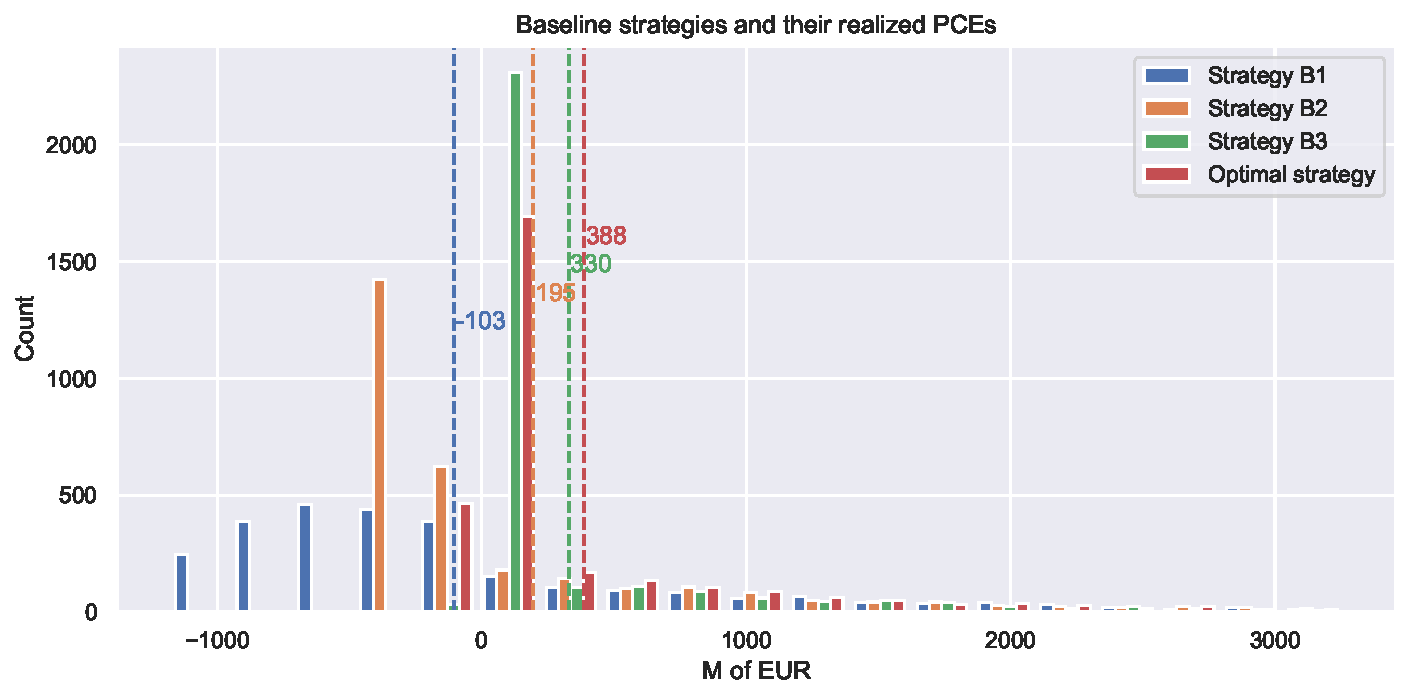
\includegraphics[scale = 0.65]{Images/MT_results_1.pdf}
		\caption{Comparison of average PCE equivalents of individual strategies, realization histograms and averages with initial settings.} 
		\label{fig:Results_init}
	\end{center}
\end{figure}



\subsection{Results - increased volatiltiy}
The second part of the simulation is exactly the same as the firs part, the only change is in increse of all price volatilities by 20\% as can be seen in table \ref{Table:init_values}. The resuls of this simualtion can be seen in figure \ref{fig:Results_increased}, while the comparison of individual results for both cases can be found in table \ref{Table:Result_comparison}
 
 
 
 \begin{figure}[htb]
 	\begin{center}
 		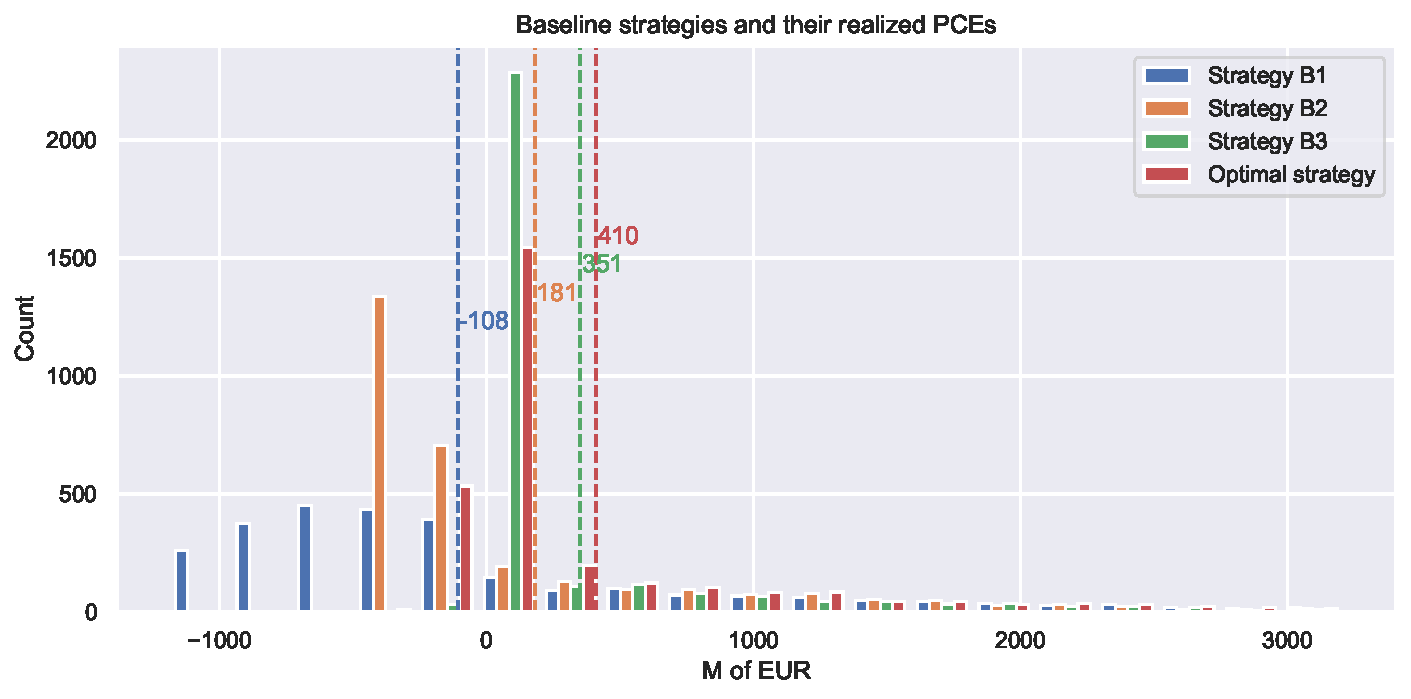
\includegraphics[scale = 0.65]{Images/MT_results_2.pdf}
 		\caption{Comparison of average PCE equivalents of individual strategies, increased volatility.} 
 		\label{fig:Results_increased}
 	\end{center}
 \end{figure}
 

 	\begin{table}
 		\begin{center}
 			\label{Table:Result_comparison}
 	\begin{tabular}{|l |r |r |r |r|} 
 		\hline
 		Setup\ Strategy &	Baseline 1 & Baseline 2 & Baseline 3 & Optimal strategy  \\  
 		\hline
 		Initial setup & -152M & 116M & 229M & 317M \\ 
 		\hline
 		Increased volatility  & -110M & 183M & 323M & 406M \\
 		\hline
 	\end{tabular}
 	\caption{Comparison of PCE for different strategies and settings.}
 	 \end{center}
 	\end{table}

 
 
 
 

\chapter{Discussion}
We believe that in the presented experiments, we have shown the usage of the SDT-based valuation technique algorithm on an example with a reasonable complexity. We have managed to cope with the uncountable state space caused by the assumption of continuous prices and also with the modelling of approximate value functions guided by the theory of ADP. 

The economical truths that we wanted to preserve from the field of capital investment bring after the experiment mixed feelings. The notion of PCE and it usage in the experiment seems to make a logical sense. However the notion of utility and risk-aversion of investors might make a better sense in the evaluation of the project as a whole. The usage of utility will be discussed in more detail below. 

\section{Value function approximation}
In the first attempts to construct the experiment for this thesis, we came up with much more complex example than the one finally presented. There were 9 elementary states, concerning for example the support of the government of renewable sources of energy which influenced the future volatility of the power prices. We also firsly introduced actions like mothballing or selling the plant for salvage value. From the study of value funciton approximations it seemed like that it will be enought to use only the linear model and choose good basis functions. But we were wrong. 

The complexity and non-linearity of the value functions is seen in the final simplified example too. It is clear now, that the option-like pattern appears, but what the future users need to keep in mind is that the complexity of the project that is to be valued will be reflected in the complexity of the value function model. 

In our case, three piecewise linear models were enough to reasonably cover the state space, but for a more complex models, there might not be such a clear patterns as we observed in our example. 

Our final choice of the example was thus simplified, so that the complexity of modelling the value funciton would not take to much attention from the main message which is the illustration of the valuation algorithm itself. 

We would like to raise a concern about the possible future adoption of the algorithm from the capital investment companies due to the complexity of the value function modelling for more real-life complex investments. 

\section{Usage of utiltiy} 
In this thesis, we wanted to preserve the notion of risk-averse investors. We did this by making the optimal decision strategy the one that maximizes the expected utility of the investor. However, when we thought deeper about the global view of investors, the real decision makers, the utility function may be used a little differently. 

We have used the utility funciton for decisions on the micro-level, when the project is being further managed. However, in reality, the group of people that make the investment decision does not usually make the further management of the project. 

On the macro level, the final valuation of a project is usually used for comparison to other investment opportunities and we believe that this is where the utility function should come into the picture. 

When looking at the results of our simulaiton, we for example see that the baseline strategy B3 is more conservative than the optimal one we derived from our algorithm. Here, we can easily imagine a very risk-averse investor which would prefer the results of strategy B3 over the optimal strategy we have derived. 

Thus, we believe there might be two utility adjustments, first on the micro-level, where the manager of the plant optimizes the utility of each action. The second utility adjustment for the valuation is for the macro level, where the board of decision makers will compare individual projects between each other.

\section{Computational complexity}
In the section ... we have talked about the computational complexity of dynamic programming. For the setup of the experiment we made (uncountable state space) the DP approach is not even theoretically possible, but wee would still like to address the computational complexity and the challenges our algorithm faces. 

We needed to compute 3 models for each of 300 time epochs. For each model we needed to have 100 state samples to cover the state space reasonably. For each state we needed to numerically compute the expected utility which was in a for of integral, to which we have also used 100 integral samples. This results in a 90 000 of state-utility pairs and 9M of integral samples created as an evolution of state with a lenght 5. The computations took several hours on a 2-core device with  16GM of RAM, where it needs to be said that the code was optimized without a special care. 

This is to say, that more complex valuation problems, might also bring with them the need for either faster hardware, or better techniques in numerical approximation of integrals and/or more robust models for the value function approximation. 



\section{Experimental results}
Even though the main focus of the experiments was to present a reasonable illustration of the valuation algorithm we can also see the individual ROA narratives in the results. 

First is the notion that uncertainty brings more value to the option-like investment. We can see this being confirmed by the higher expected PCE values for the second part of our experiment, where we increased the volatility of commodity prices. 
<Why is there an increase in the strategy B1, that should maybe not be there> 

By observing the shapes of histograms of different strategies we can also observe the narative of ROA that "options have value".  The baseline strategy B1 factually represents no options in ROA sense, we simply build the plant and run it until the end of observation period. 

The baseline strategy B2 represents the option to not run the plant when the market prices are not favorable. We can see that this option has a significant value, bringing the value of a given project from negative values to positive. 

The baseline strategy B3 represents the combination of time option (waiting for favorable commodity prices) and the option from strategy B2. We see that for our initial state, this option also brings significant value to the project. 

The final remark to the experimental results is that our intuition says that the baseline strategy B3 could be a very good approximation for the optimal strategy derived by our algorithm with a better threshold than 40 EUR. The idea is that for our simple case, the optimal strategy simply finds the best thresholds to build the first and second block. However, in comparison to B3, the optimal strategy presumably also considers the epochs left until the 300 threshold. 


\chapter{Conclusion}
The core message of this thesis is to interpret the problem of project valuation in the form of stochastic decision making. The contributions of the newly presented valuation algorithm in contrast to already existing techniques are: 
\begin{itemize}
	\item  Usage of general distributions
	\item  Theoretically any number and type of actions
	\item ... 
\end{itemize}

Furthermore, the thesis copes with the problem of computational complexity, arising as a result of high-dimensional problems, with identifying a <ADP theory> as the best fitting algorithm from the class of ADP for the problem of project valuation.

The new approach to project valuation is demonstrated on six variations of one project type, which show its real applicability in real world. First three examples confirm the expected sensitivity of the project’s value on the level of possible managerial actions, endorsing the idea that projects with higher degree of managerial action space have more value. The second trio of experiments shows how is the valuation sensitive on the choice of SDT framework. We conclude that … <probably not much> 

The limitations of this approach are: 

Finally, through the time of writing this thesis I have identified the following directions for further research as: 

\begin{itemize}
	\item ... 
\end{itemize}







\pagestyle{plain}
\bibliographystyle{plain}
\bibliography{fr}


\end{document}
